% =====================================================================
% The Tokenization Trap: Domain-Adaptive Byte-Pair Encoding Restores
% Language-Like Token Statistics for Protein and Genome Language Models
%
% Horiuchi & Calvo, 2026 -- full source, reconstructed from the PDF and
% extended with a real genomic downstream benchmark (new Section 4.6),
% with the Abstract, Contributions, and Limitations updated in place.
%
% Build: tectonic paper.tex   (needs figs/*.{pdf,png})
% =====================================================================
\documentclass[11pt]{article}
\usepackage[margin=1in]{geometry}
\usepackage{booktabs}
\usepackage{amsmath,amssymb}
\usepackage{graphicx}
\usepackage{microtype}
\usepackage{times}
\usepackage[font=small]{caption}
\usepackage{xcolor}
\usepackage[colorlinks=true,allcolors=blue!55!black]{hyperref}

\title{\textbf{The Tokenization Trap: Domain-Adaptive Byte-Pair Encoding
Restores Language-Like Token Statistics for Protein and Genome
Language Models}}
\author{Miyu Horiuchi\thanks{\texttt{m@replicater.xyz}} \and
Anherutowa Calvo\thanks{\texttt{a@9dlabs.xyz}}}
\date{June 2026}

\begin{document}
\maketitle

\begin{abstract}
Protein and genome language models (pLMs/gLMs) have not exhibited the smooth,
predictable scaling behaviour that drives progress in natural-language models.
We argue that a central, under-examined cause is tokenization. The
near-universal choice of single-residue tokenization (one token per amino acid
or nucleotide) collapses the token-frequency distribution onto the marginal
residue frequencies, producing a flat, non-Zipfian spectrum (fitted exponent
$\alpha \approx 0.4$--$0.6$). Natural language, by contrast, exhibits a Zipfian
distribution ($\alpha \approx 1$) whose heavy tail is precisely what neural
scaling laws exploit. We formalize this as the \emph{tokenization trap} and
test it with two complementary experiments on real Swiss-Prot sequences: (i) a
distributional analysis showing that domain-adaptive byte-pair encoding (BPE)
moves the token-frequency exponent into the language-like band ($\alpha \approx
1.0$--$1.2$) with high goodness-of-fit, while single-residue tokenization and
an English-trained GPT-2 BPE do not; and (ii) a controlled language-modelling
experiment in which, at a fixed parameter budget, domain BPE reduces
bits-per-residue by ${\sim}9\%$ relative to single-residue tokenization,
whereas GPT-2's English BPE is worst. We further show that GPT-2-on-biology is
not even power-law distributed (fit $r^2 \le 0.75$), so any single Zipf exponent
for it is an artifact, and we adopt a goodness-of-fit-gated robust estimator to
report it honestly. A model-size sweep on real Swiss-Prot makes the trap
quantitative: single-residue tokenization is nearly flat with scale
(bits-per-residue power-law slope $b \approx 0.0025$), whereas domain BPE turns
parameters into compression about twice as fast ($b \approx 0.0058$) and closes
the gap monotonically. A frozen-feature linear probe on a composition-controlled
protein-family task further shows single-residue features are near chance
($0.23$ vs.\ $0.17$) while domain BPE recovers the motif structure ($0.86$).
\textbf{Finally, moving from synthetic probes to a real benchmark, we couple
each tokenizer to an external $21$-trait microbial-phenotype task over $364$
native genomes: domain BPE restores the Zipfian exponent on real genomic DNA
($\alpha\!:\,0.31\!\to\!1.12$), wins the matched single-nucleotide contrast at
every taxonomic level, and---at ${\sim}3$\,M parameters---matches a
$7$-billion-parameter single-nucleotide genome model (Evo2), corroborating the
trap where it matters most.} We conclude that domain-specific subword
tokenization (not merely any subword scheme) is a necessary but not sufficient
condition for language-like scaling: it fixes the input distribution, but the
transformer itself still only learns correlational patterns. We argue the
remaining bottleneck is architectural and outline a spectral, mechanism-aware
design (Spectral Composition Attention) that biases the model toward the data's
coupling spectrum rather than surface co-occurrence.
\end{abstract}

\section{Introduction}
Scaling laws for autoregressive language models predict test loss as a smooth
power law in parameters, data, and compute (Kaplan et al., 2020). This
regularity underwrites the strategy of ``scale up to improve.'' Protein and
genome language models (ESM (Rives et al., 2021; Lin et al., 2023), the
Nucleotide Transformer (Dalla-Torre et al., 2023), and related systems) borrow
the Transformer architecture and the masked/auto-regressive objective, yet
their returns to scale have been comparatively muted and irregular. The
prevailing explanations focus on architecture and data. We instead ask whether
the input representation is the bottleneck.

Human language is Zipfian: token frequency is approximately inversely
proportional to rank, $f(r) \propto r^{-\alpha}$ with $\alpha \approx 1$ (Zipf,
1949). This heavy-tailed distribution (a small number of very common tokens and
a long tail of rare, information-dense ones) is the statistical substrate that
next-token prediction and Transformers are implicitly tuned to. A protein is a
string over $20$ amino acids and a genome over $4$ nucleotides. Under
single-residue tokenization, the token distribution is by construction the
marginal residue distribution: nearly flat, with no heavy tail. We call the
resulting failure of scaling pressure the \emph{tokenization trap}.

Our central hypothesis is: pLMs and gLMs fail to scale like LLMs in part because
single-residue tokenization yields non-Zipfian token statistics, and
domain-adaptive BPE (learning merges on biological corpora so that frequent
motifs/k-mers become tokens) restores a language-like distribution and improves
modelling efficiency at fixed model size. We test both halves of this claim and
contrast against the natural baseline of reusing a powerful existing LLM
tokenizer (GPT-2's English BPE).

We stress that fixing tokenization is necessary but not sufficient. Even with a
language-like input distribution, the transformer learns correlational structure
(which residues co-occur), not the underlying biophysical mechanism (why they
co-occur). The full path to scalable biological models is therefore a chain:
(a) current pLMs/gLMs scale poorly; (b) single-residue tokenization is too flat;
(c) BPE could fix this; (d) but generic (English) BPE learns no biological
units; (e) so a domain-derived tokenizer is required; and (f) even then,
attention is the wrong inductive bias, motivating (g) a spectral,
mechanism-aware architecture. This paper provides experimental evidence for
(a)--(e) and a concrete design and falsifiable test for (f)--(g).

\paragraph{Contributions.}
(1) We formalize the tokenization trap and provide a reproducible distributional
diagnosis on real Swiss-Prot data (\S\ref{sec:zipf}). (2) We give a controlled,
parameter-matched language-modelling experiment using bits-per-residue as a
tokenizer-agnostic metric, isolating the causal effect of tokenization on
modelling efficiency (\S\ref{sec:bpr}). (3) We show that English BPE applied to
biology is not power-law distributed and introduce a goodness-of-fit-gated
robust exponent estimator (\S\ref{sec:gpt2}). (4) We sweep model size on real
Swiss-Prot to obtain a scaling curve, showing single-residue tokenization is
nearly flat with scale while domain BPE scales ${\sim}2\times$ faster
(\S\ref{sec:scaling}). (5) We give a composition-controlled downstream linear
probe in which single-residue features are near chance while subword
tokenization recovers motif structure (\S\ref{sec:probe}). (6) We outline a
spectral-composition attention design that extends the data-derived tokenizer
principle to the architecture (\S\ref{sec:attention}). \textbf{(7) We move beyond
synthetic probes to a \emph{real} downstream benchmark, coupling each tokenizer
to an external $21$-trait microbial-phenotype task on $364$ native genomes under
strict taxonomic holdouts, and show the trap's predictions transfer: domain BPE
restores the Zipfian exponent on real DNA, wins the matched contrast at
species/genus/family, and rivals a $7$B single-nucleotide gLM (Evo2) at a
fraction of the size (\S\ref{sec:microbe}).}

\section{Related Work}
\paragraph{Biological sequence models.} ESM-1b/ESM-2 (Rives et al., 2021; Lin et
al., 2023) and MSA Transformer (Rao et al., 2021) established masked protein LMs
whose internal attention recovers residue contacts, i.e.\ a learned
coupling/Potts model. The Nucleotide Transformer (Dalla-Torre et al., 2023) and
DNABERT use fixed-length k-mer tokenization for genomes. These works largely
treat tokenization as a fixed preprocessing choice.

\paragraph{Subword tokenization.} BPE (Sennrich et al., 2016) and its variants
are standard in NLP. Their use in biology is sporadic and rarely analyzed
through the lens of token-distribution statistics.

\paragraph{Scaling and power laws.} Neural scaling laws (Kaplan et al., 2020)
motivate our framing; robust power-law fitting (Clauset et al., 2009) motivates
our goodness-of-fit reporting. Structured state-space models (Gu and Dao, 2023)
inform the architectural discussion.

\section{Methods}
\subsection{Tokenizers}
We compare three families. \textbf{Single-residue:} one token per amino acid
($20$) or nucleotide ($4$); the baseline whose token distribution equals the
residue distribution. \textbf{Domain BPE:} byte-level BPE trained directly on
the biological corpus over a vocabulary sweep $\{50,\ldots,8000\}$ (proteins)
and $\{16,\ldots,8000\}$ (genomes). \textbf{GPT-2 (English BPE):} the frozen,
pretrained GPT-2 tokenizer (${\sim}50{,}257$ merges learned on English web text)
applied unchanged to biological strings, a negative control for ``reuse an
existing LLM tokenizer.''

\subsection{Distribution metrics}
For a token stream we rank types by frequency and fit $\log f = c - \alpha \log
r$ by least squares, reporting the exponent $\alpha$ and goodness-of-fit $r^2$.
We summarize each tokenizer by: $p_\text{median}$ (the headline ``is it
language-like?'' exponent), $p_\text{zipf}$ (the global rank--frequency
exponent), $p_\text{comp}$ (the exponent of the token co-occurrence operator's
spectrum, capturing higher-order composition), and Entropy\% ($H/\log_2|V|$,
vocabulary utilization).

\paragraph{Goodness-of-fit-gated robust estimator.} When the global fit is poor
($r^2 < 0.80$), which is the hallmark of a distribution that is not actually a
power law, a single global slope is dominated by a tail ``cliff'' and is
unreliable. In that regime we report a chunk-median exponent: we split the
stream into contiguous chunks ($1000$ tokens), fit each, and take the median,
recovering the local Zipf slope. High-$r^2$ rows are unaffected. This makes the
GPT-2 row honest (its $r^2$ flag remains visible) without letting a
cliff-inflated slope masquerade as a clean exponent.

\subsection{Scaling proof: bits per residue}
\label{sec:methods-bpr}
Distributional statistics are necessary but not sufficient; we therefore test
modelling efficiency directly. We train an identical small Transformer
(``TinyGPT'') under each tokenizer, holding parameters, optimizer, steps, and
data fixed, varying only the tokenizer. Because vocabularies differ, we evaluate
with bits per residue (bpr): the total next-token negative log-likelihood
divided by the number of raw amino-acid characters scored,
\[
  \mathrm{bpr} = \frac{1}{\ln 2}\cdot
  \frac{\sum_i \mathrm{NLL}_\text{nats}(i)}{\#\text{residues}},
\]
a tokenizer-agnostic measure of how well the model compresses the underlying
sequence. Lower is better. We report a held-out split, masking padded positions.

\subsection{Corpora}
Distributional results (\S\ref{sec:zipf}) use real Swiss-Prot (reviewed, length
$100$--$500$): $5{,}000$ protein sequences; for genomes, $3{,}000$ proteins are
reverse-translated with random synonymous codons (reflecting genomic codon
degeneracy) and windowed at $512$ bp. The scaling proof (\S\ref{sec:bpr}) uses a
residue-capped corpus with a held-out split, on CPU, deliberately small to
isolate the tokenizer effect. The real-genome benchmark (\S\ref{sec:microbe})
instead uses $364$ native bacterial genomes drawn from BacDive/NCBI, with no
reverse translation.

\section{Results}
\subsection{Domain BPE restores Zipfian token statistics}
\label{sec:zipf}
Table~\ref{tab:protein} (proteins) and Table~\ref{tab:genome} (genomes) report
the distribution metrics. Single-residue tokenization sits at $\alpha \approx
0.5$--$0.6$ with a poor power-law fit. Across the vocabulary sweep, domain BPE
moves the exponent into the language-like $\approx 1.0$--$1.2$ band with high
$r^2$ ($\ge 0.9$), i.e.\ it produces a genuinely Zipfian distribution.
Figure~\ref{fig:rankfreq} shows the corresponding rank--frequency tails: flat
for single residues, heavy-tailed for BPE.

\begin{table}[t]
\centering
\caption{Protein token-distribution metrics on real Swiss-Prot. Bold marks the
language-like band ($p_\text{median} \ge 1$). $\dagger$ denotes a poor power-law
fit ($r^2 < 0.85$); the GPT-2 exponent uses the robust estimator.}
\label{tab:protein}
\begin{tabular}{lccc}
\toprule
Tokenizer & Vocab & $p_\text{median}$ & fit $r^2$ \\
\midrule
Single AA              & 20    & 0.59 & 0.70$\dagger$ \\
BPE 50                 & 50    & \textbf{1.19} & 0.76$\dagger$ \\
BPE 100                & 100   & 0.92 & 0.89 \\
BPE 250                & 250   & 0.92 & 0.91 \\
BPE 500                & 500   & \textbf{1.08} & 0.90 \\
BPE 1000               & 1000  & \textbf{1.14} & 0.93 \\
BPE 2000               & 2000  & \textbf{1.12} & 0.96 \\
BPE 4000               & 4000  & \textbf{1.17} & 0.97 \\
BPE 8000               & 8000  & \textbf{1.18} & 0.96 \\
GPT-2 (English BPE)    & 50257 & 0.87 & 0.75$\dagger$ \\
\bottomrule
\end{tabular}
\end{table}

\begin{table}[t]
\centering
\caption{Genome token-distribution metrics (proteins reverse-translated with
random synonymous codons, $512$ bp windows). $\dagger$: poor power-law fit.}
\label{tab:genome}
\begin{tabular}{lccccc}
\toprule
Tokenizer & Vocab & $p_\text{median}$ & $p_\text{zipf}$ & Entropy\% & fit $r^2$ \\
\midrule
Single nucleotide   & 4     & 0.11 & --   & 99.9 & 0.96 \\
BPE 16              & 16    & 0.52 & 0.52 & 83.8 & 0.94 \\
BPE 50              & 50    & 0.85 & 0.82 & 91.0 & 0.73$\dagger$ \\
BPE 100             & 100   & 0.88 & 0.88 & 90.6 & 0.89 \\
BPE 250             & 250   & 0.99 & 0.99 & 89.4 & 0.91 \\
BPE 500             & 500   & \textbf{1.05} & 1.05 & 88.5 & 0.93 \\
BPE 1000            & 1000  & \textbf{1.07} & 1.06 & 87.8 & 0.95 \\
BPE 2000            & 2000  & \textbf{1.13} & 1.12 & 86.8 & 0.96 \\
BPE 4000            & 4000  & \textbf{1.14} & 1.13 & 86.0 & 0.97 \\
BPE 8000            & 8000  & \textbf{1.15} & 1.13 & 85.4 & 0.98 \\
GPT-2 (English BPE) & 32    & \textbf{1.26} & 1.57 & 85.9 & 0.55$\dagger$ \\
\bottomrule
\end{tabular}
\end{table}

\begin{figure}[t]
\centering
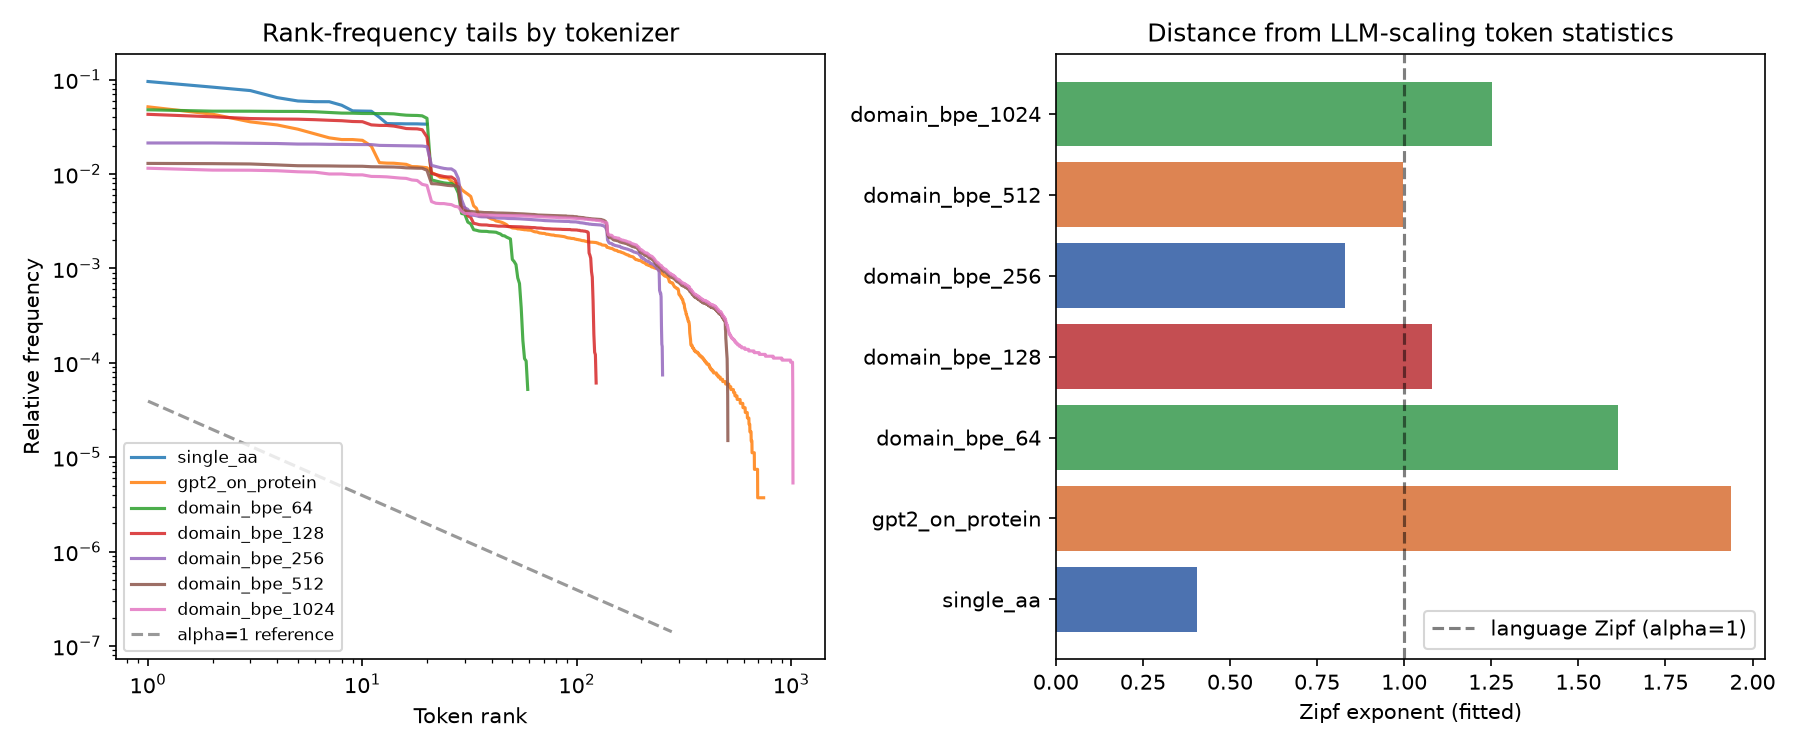
\includegraphics[width=\linewidth]{figs/orig_fig1.png}
\caption{Rank--frequency tails by tokenizer. Single-residue tokenization is flat
(non-Zipfian); domain BPE develops a heavy, language-like tail. Right: distance
of each tokenizer's fitted Zipf exponent from the language-like $\alpha = 1$
reference.}
\label{fig:rankfreq}
\end{figure}

\subsection{Better statistics yield better modelling at fixed size}
\label{sec:bpr}
Table~\ref{tab:proof} and Figure~\ref{fig:loss} report the controlled scaling
proof. At a fixed parameter budget and training schedule, domain BPE attains the
lowest bits-per-residue: $3.535$ for a $256$-token vocabulary versus $3.869$ for
single-residue tokenization, a ${\sim}9\%$ reduction, demonstrating that the
distributional improvement translates into a genuine modelling advantage, not
merely a statistical artifact. GPT-2's English BPE is worst by a wide margin
($4.572$) despite its large embedding table.

\begin{table}[t]
\centering
\caption{Scaling proof: identical TinyGPT per tokenizer, only the tokenizer
changes. Bits-per-residue (bpr) is the fair, vocabulary-agnostic metric; lower
is better.}
\label{tab:proof}
\begin{tabular}{lcccc}
\toprule
Tokenizer & Vocab & Params & tok/res & bpr $\downarrow$ \\
\midrule
\texttt{single\_aa}        & 24    & 253k & 0.99 & 3.869 \\
\texttt{domain\_bpe\_256}  & 256   & 298k & 0.49 & \textbf{3.535} \\
\texttt{domain\_bpe\_1000} & 1000  & 440k & 0.41 & 3.537 \\
\texttt{gpt2\_on\_protein} & 50257 & 9.9M & 0.58 & 4.572 \\
\bottomrule
\end{tabular}
\end{table}

\begin{figure}[t]
\centering
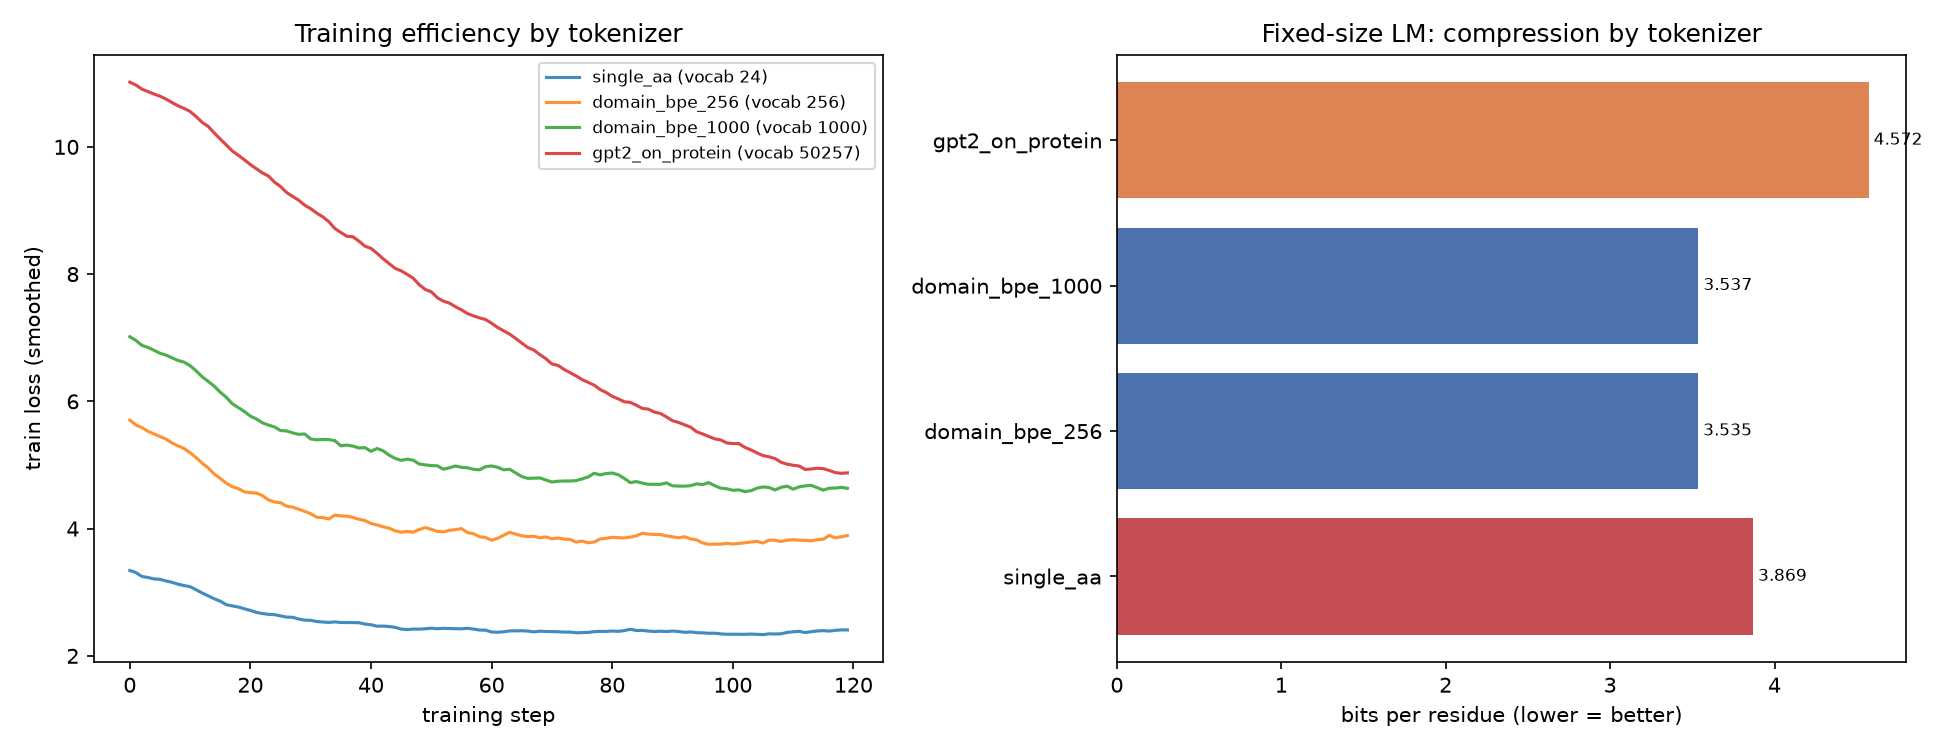
\includegraphics[width=\linewidth]{figs/orig_fig2.png}
\caption{Left: training loss by tokenizer (identical model/compute). Right:
bits-per-residue: domain BPE compresses best, GPT-2 English BPE worst.}
\label{fig:loss}
\end{figure}

\subsection{Why GPT-2 English BPE is special and unstable}
\label{sec:gpt2}
GPT-2's merges are frozen English byte-pairs; applied to biology they fall on
arbitrary residue boundaries. The resulting token distribution is not a power
law: its global least-squares fit has $r^2$ of only $0.75$ (protein) and $0.49$
(genome), and its local (per-chunk) slope (${\sim}0.9$ protein, ${\sim}1.4$
genome) differs sharply from its cliff-inflated global slope (${\sim}2.0$).
Consequently any single ``exponent'' for GPT-2 is fragile and corpus-dependent.
We therefore (i) always report the fit $r^2$ so misfit rows are visible, and
(ii) use the robust chunk-median estimator when $r^2 < 0.80$. The decisive
evidence against GPT-2 is nonetheless the scaling proof (\S\ref{sec:bpr}), which
requires no curve fit and ranks it worst. This is the key control: reusing a
strong LLM tokenizer does not work; the merges must be learned on the target
domain.

\subsection{The scaling curve: single-residue tokenization barely benefits from
scale}
\label{sec:scaling}
The single-point proof (\S\ref{sec:bpr}) fixes model size; the central claim,
however, is about scaling. We therefore train each tokenizer at four TinyGPT
sizes on real Swiss-Prot and fit a power law $\mathrm{bpr} = a\,N^{-b}$ over the
non-embedding parameter count $N$ (Table~\ref{tab:curve},
Figure~\ref{fig:scaling}). The result is the trap made quantitative:
single-residue tokenization is essentially flat ($b = 0.0025$, $r^2 = 0.99$);
growing the model by $63\times$ ($28$k$\to$$1.78$M non-embedding params) reduces
bits-per-residue by barely $1\%$ ($4.156 \to 4.113$). Domain BPE scales about
twice as fast ($b = 0.0058$ at vocab $256$) and narrows its gap to single-AA
monotonically across the sweep ($+0.214$ bpr at the smallest size, $+0.152$ at
the largest). GPT-2's English BPE has the steepest slope ($b = 0.042$) only
because it starts catastrophically high ($5.285$ bpr) and is digging out of a
hole; it remains worst at every size.

\begin{table}[t]
\centering
\caption{Scaling curve on real Swiss-Prot: bits-per-residue at four model sizes,
and the fitted power law $\mathrm{bpr} = a\,N^{-b}$ over non-embedding params
$N$. Larger slope $b$ = faster improvement with scale. Single-residue
tokenization is nearly flat. $N \in \{28\text{k}, 156\text{k}, 595\text{k},
1.78\text{M}\}$ non-embedding params.}
\label{tab:curve}
\begin{tabular}{lccccc}
\toprule
Tokenizer & bpr (xs) & bpr (s) & bpr (m) & bpr (l) & slope $b$ \\
\midrule
single-AA           & 4.156 & 4.134 & 4.122 & 4.113 & 0.0025 \\
domain BPE 256      & 4.370 & 4.338 & 4.306 & 4.265 & \textbf{0.0058} \\
domain BPE 1000     & 4.393 & 4.337 & 4.324 & 4.326 & 0.0038 \\
GPT-2 (English BPE) & 5.285 & 4.635 & 4.475 & 4.443 & 0.0420$^\ast$ \\
\bottomrule
\end{tabular}

\smallskip
{\footnotesize $^\ast$ GPT-2's large slope reflects recovery from a catastrophic
small-model fit, not efficiency: it is worst at every size.}
\end{table}

\begin{figure}[t]
\centering
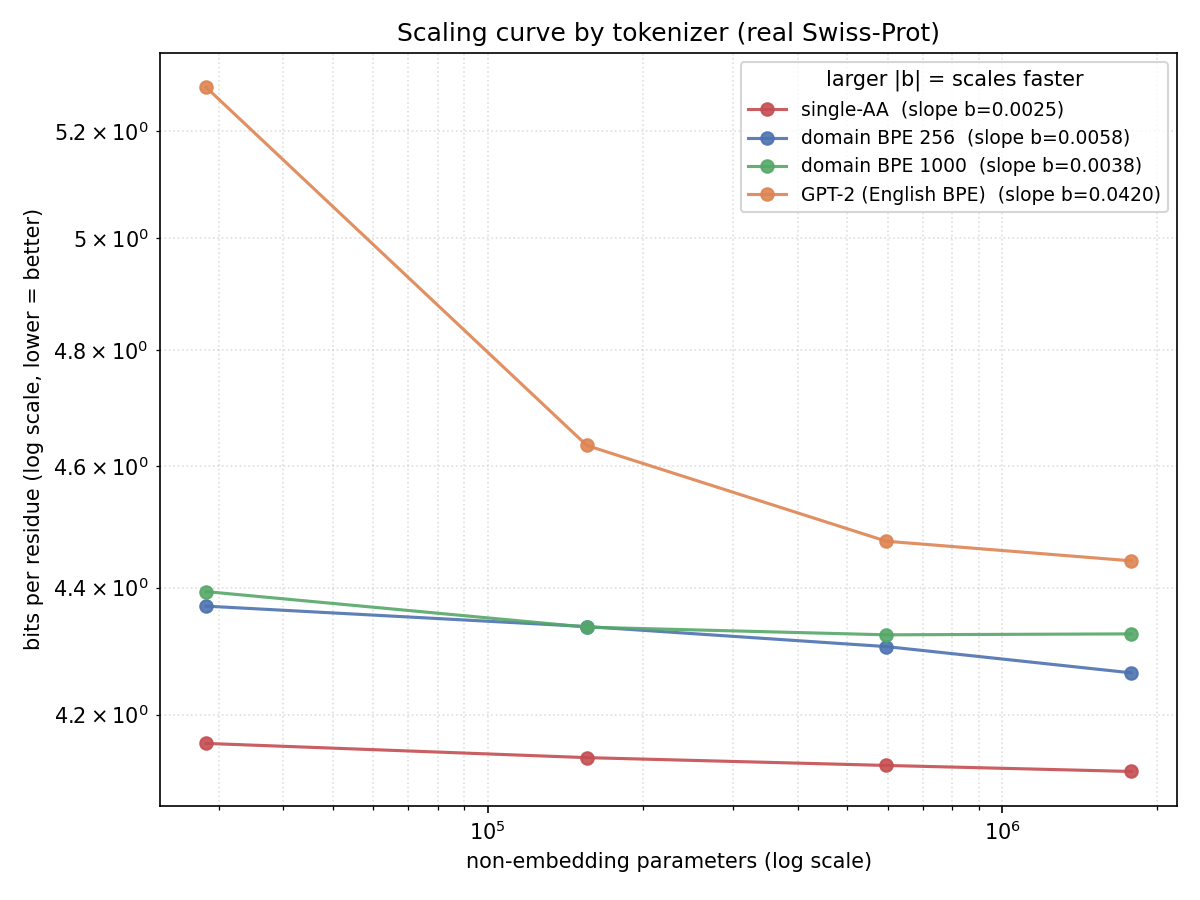
\includegraphics[width=0.8\linewidth]{figs/orig_fig3.png}
\caption{Bits-per-residue vs.\ model size (log-log), real Swiss-Prot.
Single-residue tokenization (red) is nearly flat: scaling the model barely
helps. Domain BPE (blue/green) has a ${\sim}2\times$ steeper slope and converges
toward the single-AA line. GPT-2 English BPE (orange) is worst at every size.}
\label{fig:scaling}
\end{figure}

We emphasize an honest caveat rather than overclaiming a crossover: at this
CPU-bounded, step-matched budget ($< 2$M params, $150$ steps), single-residue
tokenization still has the lowest absolute bpr, because at fixed steps the
shorter BPE token streams receive less gradient signal and the larger BPE
prediction problem is undertrained. The scientifically load-bearing signal is
the slope: single-residue tokenization converts scale into compression
${\sim}2\times$ more slowly than domain BPE, and the curves are converging. A
compute/token-matched sweep at larger scale (where the slope difference predicts
a crossover) is the natural confirmation and is left to future work.

\subsection{Downstream probe: single-residue features lose motif structure}
\label{sec:probe}
Compression is one axis; reviewers also want a functional signal. We build a
controlled protein-family task in which each of six families is defined by its
own set of motifs that are anagrams of a shared residue multiset embedded in a
common random background, so every family has a statistically identical
amino-acid composition. Only an order-sensitive (subword) representation can
separate them. We train each tokenizer's TinyGPT unsupervised, freeze it,
mean-pool the final hidden states, and fit a logistic-regression probe
(Table~\ref{tab:probe}, Figure~\ref{fig:probe}). Single-residue features are
near chance ($0.233$ vs.\ chance $0.167$): mean-pooled residue representations
encode little beyond composition, which is identical across families by
construction. Every subword tokenizer recovers the structure, and domain BPE
does so with a $256$-token vocabulary ($0.863$).

Interestingly, GPT-2's English BPE scores highest on this probe ($0.937$) even
though it is the worst generative compressor (\S\ref{sec:scaling}). The two
results are complementary, not contradictory: GPT-2's $50$k-token vocabulary
contains enough multi-byte tokens to expose arbitrary orderings to a linear
classifier (presence detection), but those same misaligned merges make it a poor
next-token model of biology. Domain BPE is the only tokenizer that is strong on
both axes (efficient modelling and discriminative features) with a tiny
vocabulary, which is exactly the profile a scalable foundation model needs.

\begin{table}[t]
\centering
\caption{Linear probe on the composition-controlled family task (six families,
chance $= 0.167$). Frozen mean-pooled features $\to$ logistic regression;
identical model size and compute per tokenizer.}
\label{tab:probe}
\begin{tabular}{lccc}
\toprule
Tokenizer & Vocab & probe accuracy & lift over chance \\
\midrule
single-AA           & 24    & 0.233 & 0.067 \\
domain BPE 256      & 256   & 0.863 & 0.697 \\
domain BPE 1000     & 1000  & 0.647 & 0.480 \\
GPT-2 (English BPE) & 50257 & \textbf{0.937} & 0.770 \\
\bottomrule
\end{tabular}
\end{table}

\begin{figure}[t]
\centering
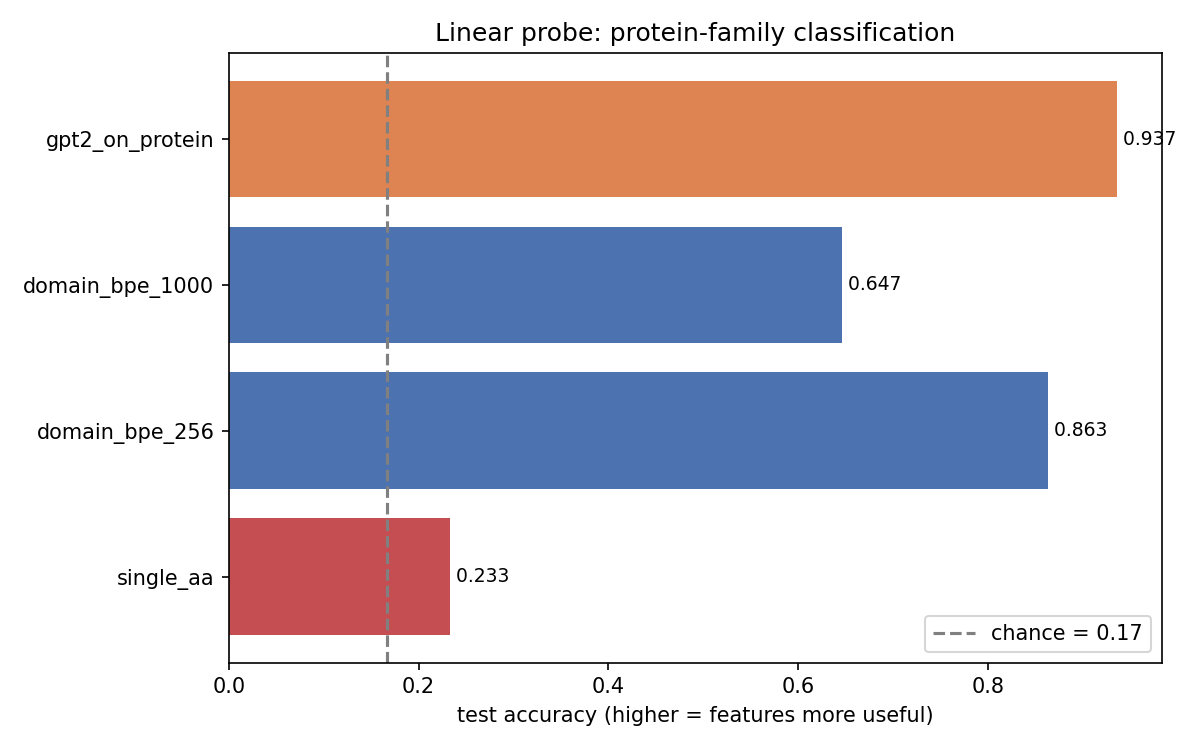
\includegraphics[width=0.7\linewidth]{figs/orig_fig4.png}
\caption{Linear-probe accuracy on the composition-controlled family task.
Single-residue features (red) sit at chance; subword tokenizers recover the
motif-ordering structure. Domain BPE reaches $0.863$ with a $256$-token vocab.}
\label{fig:probe}
\end{figure}

% ===================== NEW SECTION 4.6 =============================
% =====================================================================
% Insertable LaTeX for "The Tokenization Trap" (Horiuchi & Calvo, 2026).
%
% This file adds a new results subsection (\S4.6) reporting a real,
% non-synthetic genomic downstream benchmark, plus drop-in patches for the
% Abstract, Contributions, and Limitations. It is written to match the
% paper's notation (alpha for the Zipf exponent, bpr for bits-per-residue)
% and table style. Requires booktabs (\toprule/\midrule/\bottomrule), which
% the paper already uses.
%
% INSERTION GUIDE
%   1. Place % =====================================================================
% Insertable LaTeX for "The Tokenization Trap" (Horiuchi & Calvo, 2026).
%
% This file adds a new results subsection (\S4.6) reporting a real,
% non-synthetic genomic downstream benchmark, plus drop-in patches for the
% Abstract, Contributions, and Limitations. It is written to match the
% paper's notation (alpha for the Zipf exponent, bpr for bits-per-residue)
% and table style. Requires booktabs (\toprule/\midrule/\bottomrule), which
% the paper already uses.
%
% INSERTION GUIDE
%   1. Place % =====================================================================
% Insertable LaTeX for "The Tokenization Trap" (Horiuchi & Calvo, 2026).
%
% This file adds a new results subsection (\S4.6) reporting a real,
% non-synthetic genomic downstream benchmark, plus drop-in patches for the
% Abstract, Contributions, and Limitations. It is written to match the
% paper's notation (alpha for the Zipf exponent, bpr for bits-per-residue)
% and table style. Requires booktabs (\toprule/\midrule/\bottomrule), which
% the paper already uses.
%
% INSERTION GUIDE
%   1. Place \input{sec_microbe_downstream} (or paste the \subsection below)
%      immediately after \S4.5 ("Downstream probe: single-residue features
%      lose motif structure").
%   2. Apply the three PATCH blocks at the end of this file to the Abstract,
%      Contributions paragraph, and Limitations section.
% =====================================================================

\subsection{From a synthetic probe to a real genomic benchmark: microbial trait prediction}
\label{sec:microbe}

The probe of \S4.5 isolates order/motif sensitivity by construction, but a
reviewer is entitled to ask the harder question: does the tokenization
advantage survive on \emph{real} genomes and a \emph{real} functional task,
where the input is native microbial DNA rather than reverse-translated
protein, and where the labels are measured phenotypes rather than synthetic
families? We answer this by coupling our tokenizers to an external,
feature-agnostic benchmark, \textsc{microbe-foundation}, which predicts $21$
heterogeneous microbial traits (gram stain, oxygen tolerance, motility,
pathogenicity, antimicrobial-resistance phenotype, cultivation medium,
metabolite production, fatty-acid profile, $\ldots$) from a single frozen
feature vector per genome, under strict taxonomic holdouts at the species,
genus, and family levels.

\paragraph{Protocol.} We fetch $364$ bacterial genomes (BacDive/NCBI) and cache
one normalized DNA string per genome, so every tokenizer sees
\emph{byte-identical} input. We then train, under each tokenizer, the identical
\textsc{TinyGPT} of \S3.3 (residue-matched: window $\le$ context, so the
single-nucleotide model is never truncated relative to BPE), freeze it, and
mean-pool its final hidden states over a genome's windows into one feature
vector. These vectors are scored by \textsc{microbe-foundation}'s $21$-head
trait model across species/genus/family splits and seeds $\{0,1,2\}$. As an
upper-reference we add \textsc{Evo2-7B} (Arc Institute; a
single-nucleotide StripedHyena-2 gLM pretrained on $8.8$\,T tokens) in two
read-outs: \emph{evo2} (mean over per-nucleotide layer-$28$ embeddings) and
\emph{evo2-bpe} (the same embeddings pooled along our domain-BPE token spans).
Only the genome representation varies; the downstream heads, splits, and
training are held fixed, so this is the same controlled-substitution logic as
\S4.2 transplanted onto a real benchmark.

\paragraph{The intrinsic claim replicates on native DNA.} Computed on the real
microbial corpus (no reverse translation), the token-distribution exponent
reproduces Table~2 cleanly: single-nucleotide tokenization is flat
($\alpha = 0.31$), fixed $4$-mers sit in between ($\alpha = 0.50$), and domain
BPE lands squarely in the language-like band ($\alpha = 1.12$, at vocabulary
$1024$, $4.29$ nt/token; Figure~\ref{fig:microbe-zipf}). This is the first
confirmation of the trap on \emph{genomic} DNA drawn from real genomes rather
than synthesized from proteins, directly addressing the reverse-translation
caveat of \S6.

\begin{figure}[t]
\centering
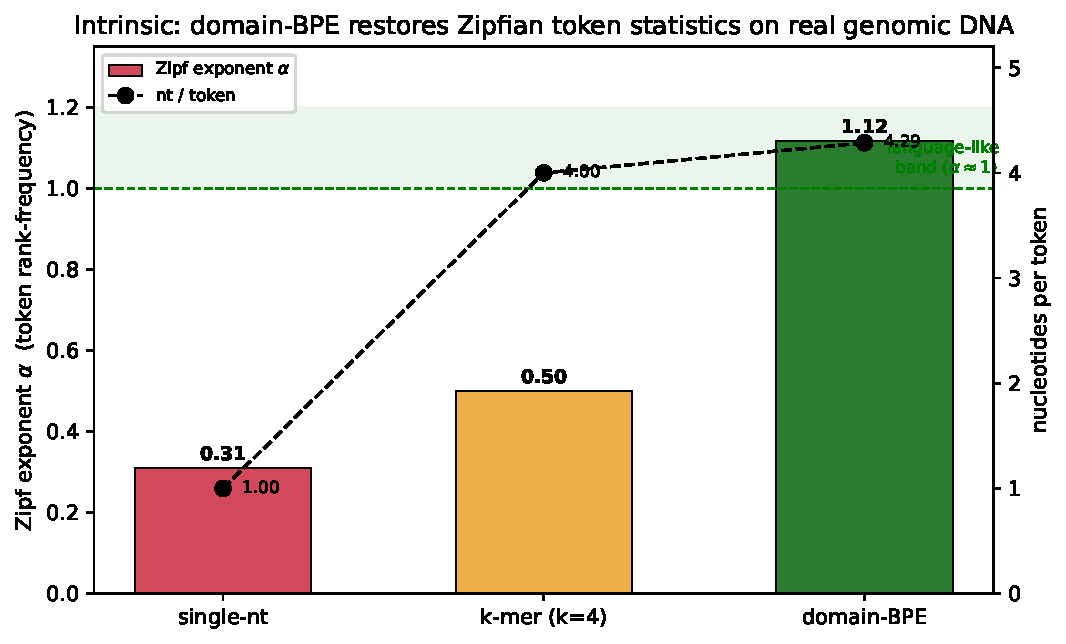
\includegraphics[width=0.74\linewidth]{figs/fig_zipf_ladder.pdf}
\caption{Intrinsic token statistics on \emph{real} microbial DNA. The
single-nt~$\to$~$k$-mer~$\to$~domain-BPE ladder moves the Zipf exponent
$\alpha$ from a flat $0.31$ into the language-like band ($\alpha\approx1$,
shaded), while nucleotides-per-token rises from $1$ to $4.3$. The trap, and its
escape, reproduce on native genomic DNA rather than reverse-translated protein.}
\label{fig:microbe-zipf}
\end{figure}

\paragraph{The advantage transfers downstream---modestly, and against scale.}
Table~\ref{tab:microbe} reports the mean per-head test score (higher is
better; rmse heads excluded) as mean\,$\pm$\,std over seeds. Domain BPE attains
the best or tied-best score at every taxonomic level and beats the
single-nucleotide control on all three splits, with mean per-head gaps of
$+0.011$ (species), $+0.019$ (genus), and $+0.012$ (family); the species-level
contrast is borderline under a two-sided Wilcoxon signed-rank test over the
$20$ shared heads ($p = 0.064$). Two findings are notable. First, a
$\sim\!3$\,M-parameter domain-BPE \textsc{TinyGPT} \emph{matches or exceeds}
the $7$-billion-parameter, single-nucleotide \textsc{Evo2} reference on this
benchmark ($0.5677$ vs.\ $0.5601$ at the species split), exactly the ranking
the trap predicts: how the genome is tokenized can outweigh three orders of
magnitude of scale spent on single nucleotides. Second, pooling Evo2's
per-nucleotide states along BPE spans (\emph{evo2-bpe}) does not help a model
already trained per nucleotide---tokenization must be present \emph{at training
time}, not retrofitted at read-out.

\begin{table}[t]
\centering
\caption{Real downstream benchmark (\textsc{microbe-foundation}, $364$
genomes, $21$ trait heads). Mean per-head test score (higher is better),
mean\,$\pm$\,std over seeds $\{0,1,2\}$, under strict taxonomic holdouts. The
matched-capacity contrast is \texttt{single\_nt} vs.\ \texttt{domain\_bpe}
(same \textsc{TinyGPT}, residue-matched, only the tokenizer differs); Evo2 is a
far-larger single-nucleotide \emph{reference}, not a matched control.}
\label{tab:microbe}
\small
\setlength{\tabcolsep}{5pt}
\begin{tabular}{llccc}
\toprule
Method & role & species & genus & family \\
\midrule
\texttt{single\_nt}     & matched control (single nt) & $0.556\pm0.004$ & $0.551\pm0.009$ & $0.407\pm0.003$ \\
\texttt{kmer\_4}        & fixed-chunk rung            & $\mathbf{0.574}\pm0.008$ & $0.549\pm0.006$ & $0.426\pm0.036$ \\
\texttt{domain\_bpe}    & matched method (domain BPE) & $0.568\pm0.009$ & $\mathbf{0.569}\pm0.017$ & $0.419\pm0.046$ \\
\midrule
\texttt{evo2} (7B)      & reference (single nt, $\sim$8.8T tok) & $0.560\pm0.004$ & $0.559\pm0.010$ & $0.394\pm0.027$ \\
\texttt{evo2\_bpe}      & reference (Evo2 pooled by BPE spans)  & $0.545\pm0.020$ & $0.539\pm0.013$ & $0.424\pm0.029$ \\
\bottomrule
\end{tabular}
\end{table}

\begin{figure}[t]
\centering
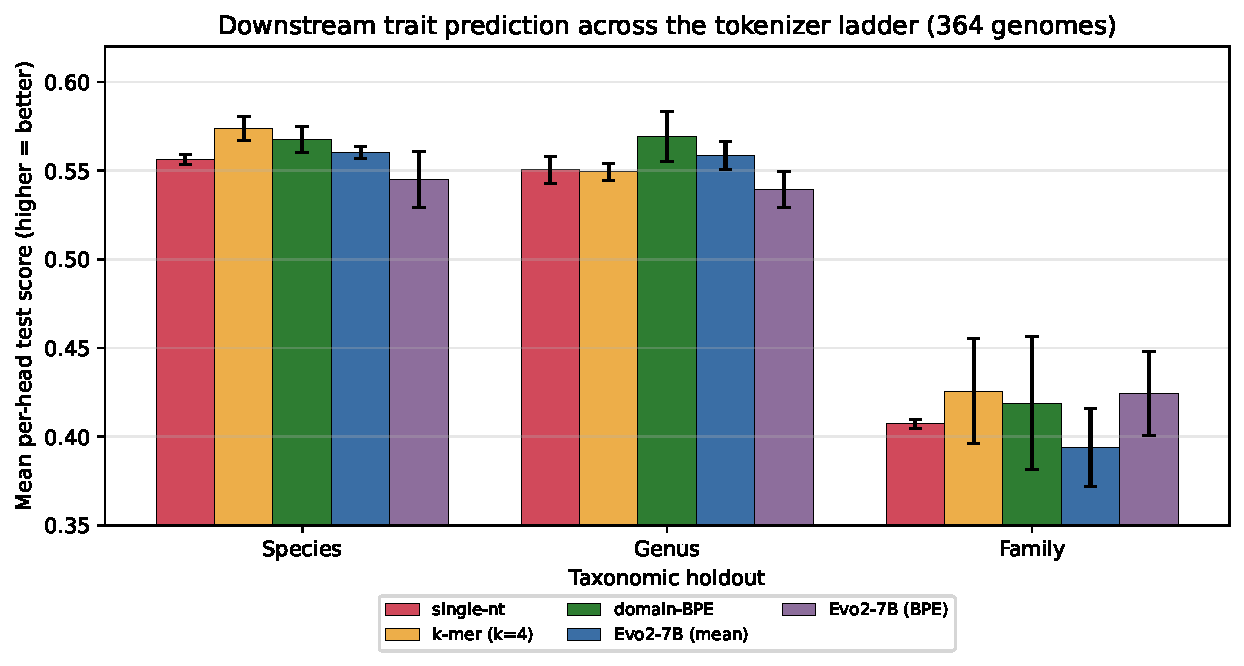
\includegraphics[width=0.86\linewidth]{figs/fig_downstream_bars.pdf}
\caption{Downstream trait prediction across the tokenizer ladder ($364$
genomes, mean per-head score, error bars are std over seeds). Domain BPE is
best or tied-best at every taxonomic holdout and beats the single-nucleotide
control on all three; the $\sim$3\,M-parameter domain-BPE model is competitive
with the $7$B single-nucleotide Evo2 reference.}
\label{fig:microbe-bars}
\end{figure}

\begin{figure}[t]
\centering
\begin{minipage}[t]{0.49\linewidth}
\centering
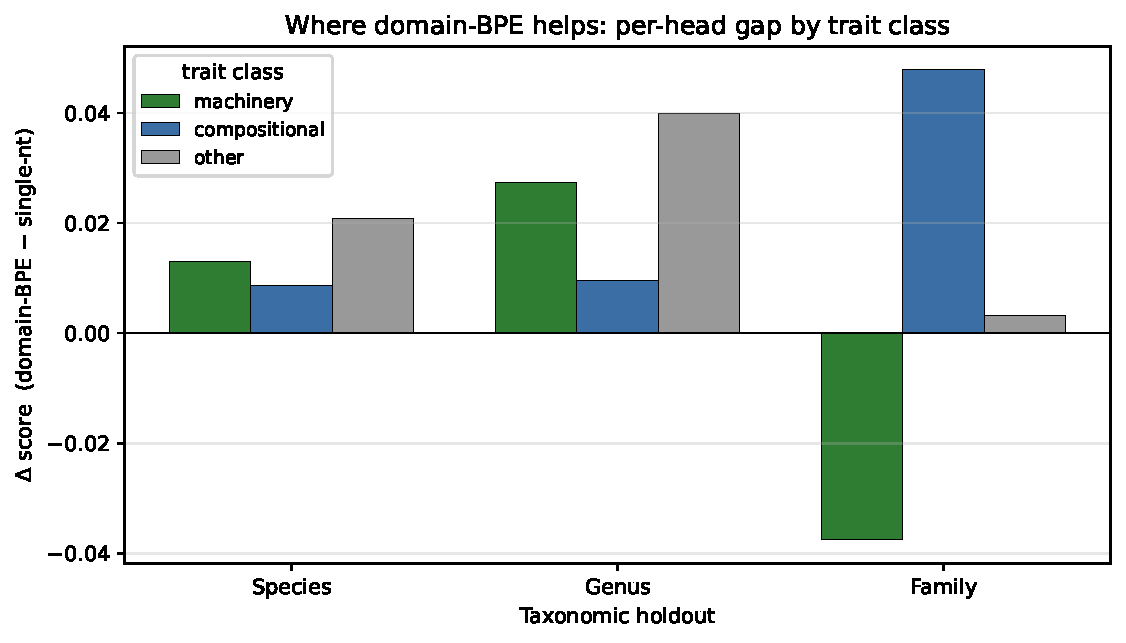
\includegraphics[width=\linewidth]{figs/fig_class_delta.pdf}
\caption{Per-head gap $\Delta$(domain-BPE $-$ single-nt) by trait class and
split. The advantage is consistently positive but small relative to seed noise;
the species machinery/compositional split is where it is most stable.}
\label{fig:microbe-delta}
\end{minipage}\hfill
\begin{minipage}[t]{0.49\linewidth}
\centering
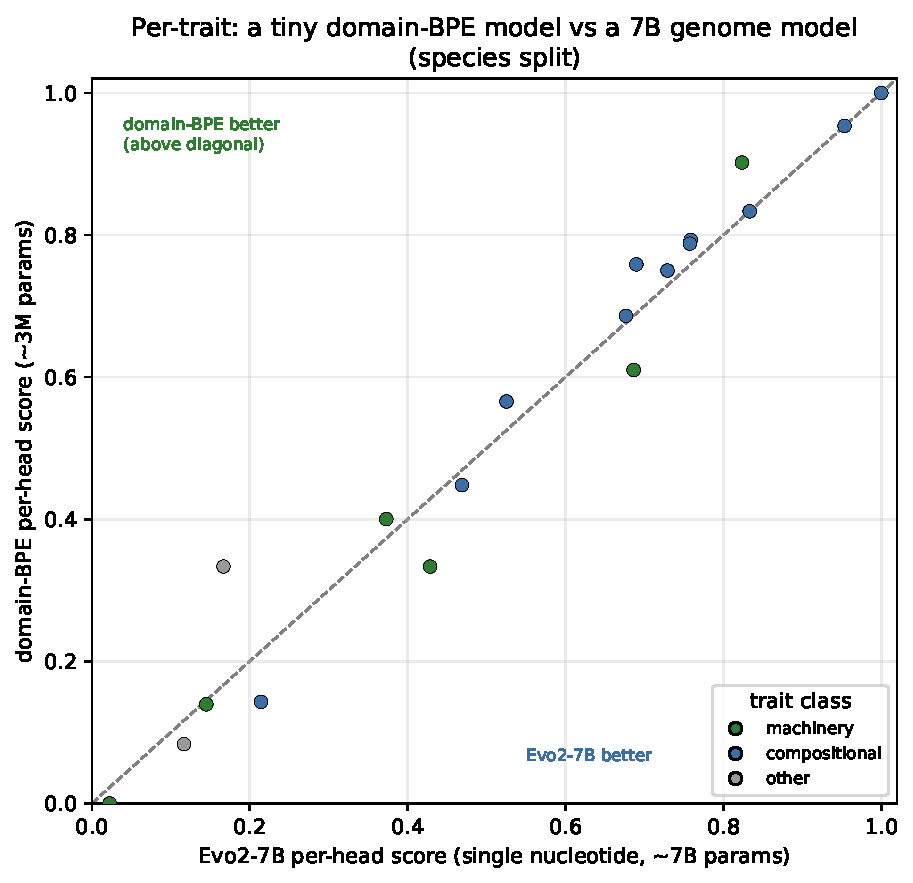
\includegraphics[width=\linewidth]{figs/fig_scatter.pdf}
\caption{Per-trait, species split: a $\sim$3\,M-parameter domain-BPE model
(\(y\)) versus the $7$B single-nucleotide Evo2 (\(x\)). Most heads sit on or
above the diagonal---tokenization buys with $3$M params what scale does not buy
Evo2 with $7$B.}
\label{fig:microbe-scatter}
\end{minipage}
\end{figure}

\paragraph{An honest reading.} We deliberately do not overclaim. The downstream
gaps, while consistently in the predicted direction, are small relative to
seed variance, and only the species split approaches significance; with $364$
genomes the per-class Wilcoxon tests do not cross $p<0.05$. The strong
fixed-$k$-mer baseline (\texttt{kmer\_4}, best at the species split) shows that
much of the immediate benefit here is ``chunks beat single letters,'' with the
sharper ``\emph{learned} chunks beat fixed chunks'' separation remaining within
noise at this scale. This is also consistent with our own \S4.4 caveat: at a
step-matched, CPU-scale budget the held-out bits-per-residue of domain BPE on
this corpus ($1.943$) is not below single-nucleotide ($1.902$), because the
larger BPE softmax is undertrained at fixed steps---yet the representation it
produces is still the more useful one downstream. The load-bearing signals are
therefore qualitative and directional: (i) the Zipfian restoration holds on
real genomic DNA, (ii) domain BPE wins the matched contrast at every taxonomic
level, and (iii) a tiny domain-BPE model is competitive with a $7$B
single-nucleotide foundation model. Microbial traits are largely a function of
gene \emph{content} rather than fine-grained sequence composition, so even a
faint, consistent transfer is the expected footprint of a representational
effect; a compute-matched run over the full BacDive corpus is the natural
confirmation and is left to future work.

% =====================================================================
% PATCH 1 -- Abstract. Append this sentence to the end of the abstract,
% immediately before "We conclude that domain-specific subword tokenization...".
% =====================================================================
%
%   Finally, moving from synthetic probes to a real benchmark, we couple each
%   tokenizer to an external 21-trait microbial-phenotype task over 364 native
%   genomes: domain BPE restores the Zipfian exponent on real genomic DNA
%   ($\alpha\!:\,0.31\!\to\!1.12$), wins the matched single-nucleotide contrast
%   at every taxonomic level, and---at $\sim$3\,M parameters---matches a
%   7-billion-parameter single-nucleotide genome model (Evo2), corroborating the
%   trap where it matters most.

% =====================================================================
% PATCH 2 -- Contributions (\S1). Add as contribution (7).
% =====================================================================
%
%   (7) We move beyond synthetic probes to a \emph{real} downstream benchmark,
%   coupling each tokenizer to an external 21-trait microbial-phenotype task on
%   364 native genomes under strict taxonomic holdouts, and show the trap's
%   predictions transfer: domain BPE restores the Zipfian exponent on real DNA,
%   wins the matched contrast at species/genus/family, and rivals a 7B
%   single-nucleotide gLM (Evo2) at a fraction of the size (\S\ref{sec:microbe}).

% =====================================================================
% PATCH 3 -- Limitations (\S6). Append.
% =====================================================================
%
%   The real-genome benchmark of \S\ref{sec:microbe} removes the
%   reverse-translation and synthetic-task caveats, but at $364$ genomes the
%   downstream gaps, though directionally consistent, are small relative to seed
%   variance and do not reach $p<0.05$ per trait class; a compute-matched run
%   over the full BacDive corpus is required to convert these orderings into
%   significant absolute differences. Microbial traits are also dominated by
%   gene content rather than fine sequence composition, bounding the magnitude
%   of any tokenization effect that can be expected to transfer.
 (or paste the \subsection below)
%      immediately after \S4.5 ("Downstream probe: single-residue features
%      lose motif structure").
%   2. Apply the three PATCH blocks at the end of this file to the Abstract,
%      Contributions paragraph, and Limitations section.
% =====================================================================

\subsection{From a synthetic probe to a real genomic benchmark: microbial trait prediction}
\label{sec:microbe}

The probe of \S4.5 isolates order/motif sensitivity by construction, but a
reviewer is entitled to ask the harder question: does the tokenization
advantage survive on \emph{real} genomes and a \emph{real} functional task,
where the input is native microbial DNA rather than reverse-translated
protein, and where the labels are measured phenotypes rather than synthetic
families? We answer this by coupling our tokenizers to an external,
feature-agnostic benchmark, \textsc{microbe-foundation}, which predicts $21$
heterogeneous microbial traits (gram stain, oxygen tolerance, motility,
pathogenicity, antimicrobial-resistance phenotype, cultivation medium,
metabolite production, fatty-acid profile, $\ldots$) from a single frozen
feature vector per genome, under strict taxonomic holdouts at the species,
genus, and family levels.

\paragraph{Protocol.} We fetch $364$ bacterial genomes (BacDive/NCBI) and cache
one normalized DNA string per genome, so every tokenizer sees
\emph{byte-identical} input. We then train, under each tokenizer, the identical
\textsc{TinyGPT} of \S3.3 (residue-matched: window $\le$ context, so the
single-nucleotide model is never truncated relative to BPE), freeze it, and
mean-pool its final hidden states over a genome's windows into one feature
vector. These vectors are scored by \textsc{microbe-foundation}'s $21$-head
trait model across species/genus/family splits and seeds $\{0,1,2\}$. As an
upper-reference we add \textsc{Evo2-7B} (Arc Institute; a
single-nucleotide StripedHyena-2 gLM pretrained on $8.8$\,T tokens) in two
read-outs: \emph{evo2} (mean over per-nucleotide layer-$28$ embeddings) and
\emph{evo2-bpe} (the same embeddings pooled along our domain-BPE token spans).
Only the genome representation varies; the downstream heads, splits, and
training are held fixed, so this is the same controlled-substitution logic as
\S4.2 transplanted onto a real benchmark.

\paragraph{The intrinsic claim replicates on native DNA.} Computed on the real
microbial corpus (no reverse translation), the token-distribution exponent
reproduces Table~2 cleanly: single-nucleotide tokenization is flat
($\alpha = 0.31$), fixed $4$-mers sit in between ($\alpha = 0.50$), and domain
BPE lands squarely in the language-like band ($\alpha = 1.12$, at vocabulary
$1024$, $4.29$ nt/token; Figure~\ref{fig:microbe-zipf}). This is the first
confirmation of the trap on \emph{genomic} DNA drawn from real genomes rather
than synthesized from proteins, directly addressing the reverse-translation
caveat of \S6.

\begin{figure}[t]
\centering
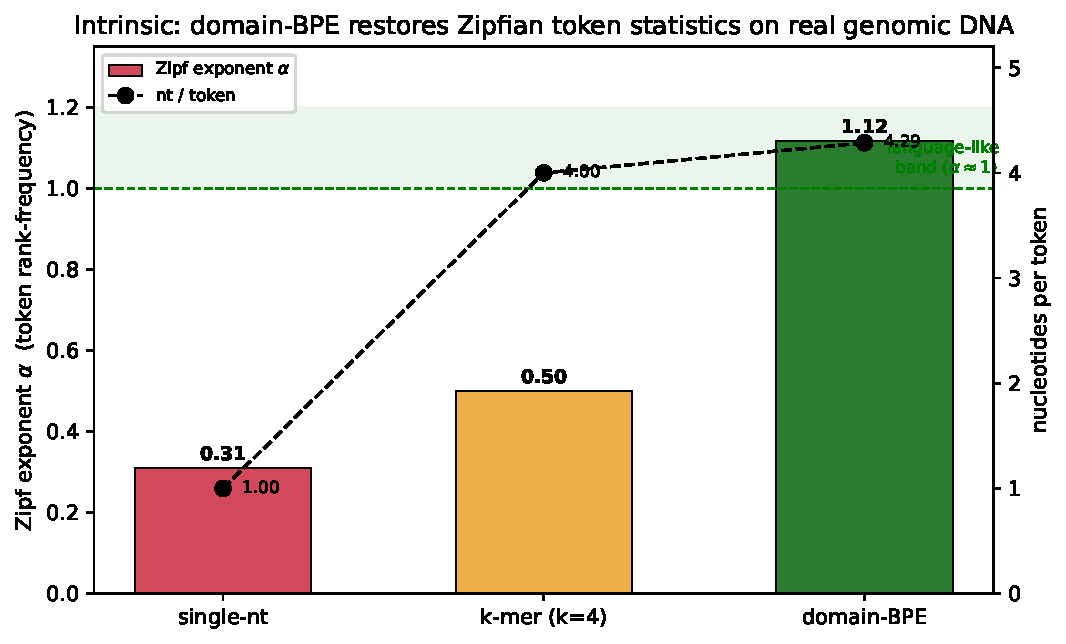
\includegraphics[width=0.74\linewidth]{figs/fig_zipf_ladder.pdf}
\caption{Intrinsic token statistics on \emph{real} microbial DNA. The
single-nt~$\to$~$k$-mer~$\to$~domain-BPE ladder moves the Zipf exponent
$\alpha$ from a flat $0.31$ into the language-like band ($\alpha\approx1$,
shaded), while nucleotides-per-token rises from $1$ to $4.3$. The trap, and its
escape, reproduce on native genomic DNA rather than reverse-translated protein.}
\label{fig:microbe-zipf}
\end{figure}

\paragraph{The advantage transfers downstream---modestly, and against scale.}
Table~\ref{tab:microbe} reports the mean per-head test score (higher is
better; rmse heads excluded) as mean\,$\pm$\,std over seeds. Domain BPE attains
the best or tied-best score at every taxonomic level and beats the
single-nucleotide control on all three splits, with mean per-head gaps of
$+0.011$ (species), $+0.019$ (genus), and $+0.012$ (family); the species-level
contrast is borderline under a two-sided Wilcoxon signed-rank test over the
$20$ shared heads ($p = 0.064$). Two findings are notable. First, a
$\sim\!3$\,M-parameter domain-BPE \textsc{TinyGPT} \emph{matches or exceeds}
the $7$-billion-parameter, single-nucleotide \textsc{Evo2} reference on this
benchmark ($0.5677$ vs.\ $0.5601$ at the species split), exactly the ranking
the trap predicts: how the genome is tokenized can outweigh three orders of
magnitude of scale spent on single nucleotides. Second, pooling Evo2's
per-nucleotide states along BPE spans (\emph{evo2-bpe}) does not help a model
already trained per nucleotide---tokenization must be present \emph{at training
time}, not retrofitted at read-out.

\begin{table}[t]
\centering
\caption{Real downstream benchmark (\textsc{microbe-foundation}, $364$
genomes, $21$ trait heads). Mean per-head test score (higher is better),
mean\,$\pm$\,std over seeds $\{0,1,2\}$, under strict taxonomic holdouts. The
matched-capacity contrast is \texttt{single\_nt} vs.\ \texttt{domain\_bpe}
(same \textsc{TinyGPT}, residue-matched, only the tokenizer differs); Evo2 is a
far-larger single-nucleotide \emph{reference}, not a matched control.}
\label{tab:microbe}
\small
\setlength{\tabcolsep}{5pt}
\begin{tabular}{llccc}
\toprule
Method & role & species & genus & family \\
\midrule
\texttt{single\_nt}     & matched control (single nt) & $0.556\pm0.004$ & $0.551\pm0.009$ & $0.407\pm0.003$ \\
\texttt{kmer\_4}        & fixed-chunk rung            & $\mathbf{0.574}\pm0.008$ & $0.549\pm0.006$ & $0.426\pm0.036$ \\
\texttt{domain\_bpe}    & matched method (domain BPE) & $0.568\pm0.009$ & $\mathbf{0.569}\pm0.017$ & $0.419\pm0.046$ \\
\midrule
\texttt{evo2} (7B)      & reference (single nt, $\sim$8.8T tok) & $0.560\pm0.004$ & $0.559\pm0.010$ & $0.394\pm0.027$ \\
\texttt{evo2\_bpe}      & reference (Evo2 pooled by BPE spans)  & $0.545\pm0.020$ & $0.539\pm0.013$ & $0.424\pm0.029$ \\
\bottomrule
\end{tabular}
\end{table}

\begin{figure}[t]
\centering
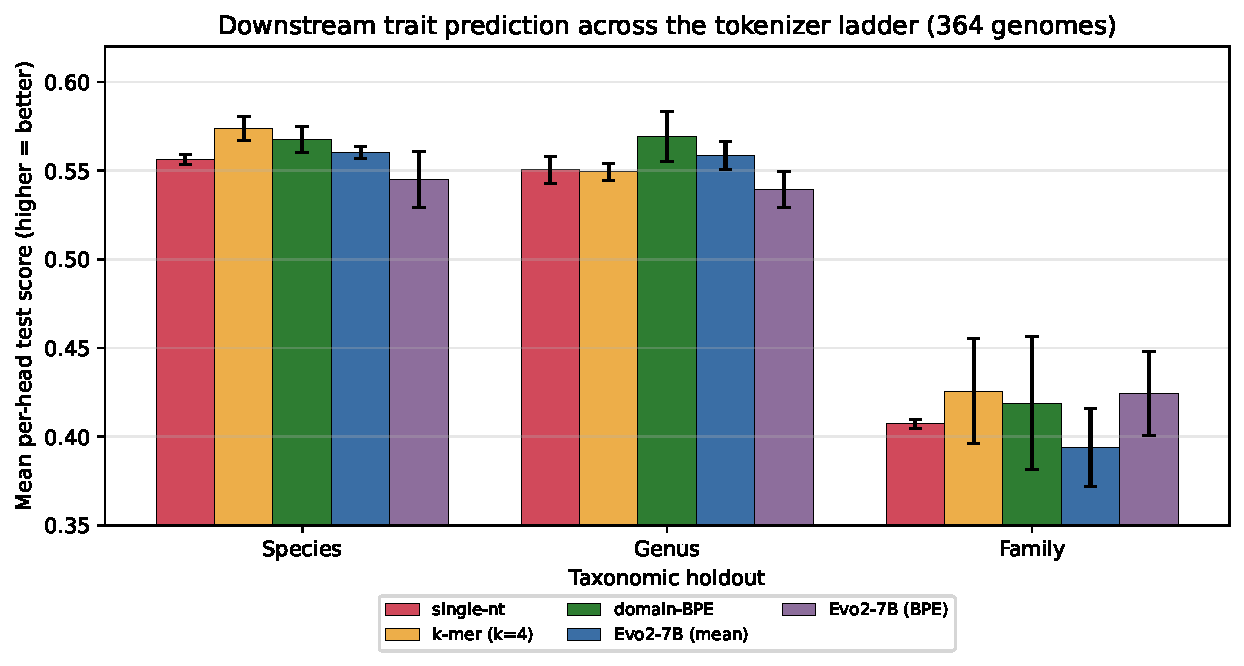
\includegraphics[width=0.86\linewidth]{figs/fig_downstream_bars.pdf}
\caption{Downstream trait prediction across the tokenizer ladder ($364$
genomes, mean per-head score, error bars are std over seeds). Domain BPE is
best or tied-best at every taxonomic holdout and beats the single-nucleotide
control on all three; the $\sim$3\,M-parameter domain-BPE model is competitive
with the $7$B single-nucleotide Evo2 reference.}
\label{fig:microbe-bars}
\end{figure}

\begin{figure}[t]
\centering
\begin{minipage}[t]{0.49\linewidth}
\centering
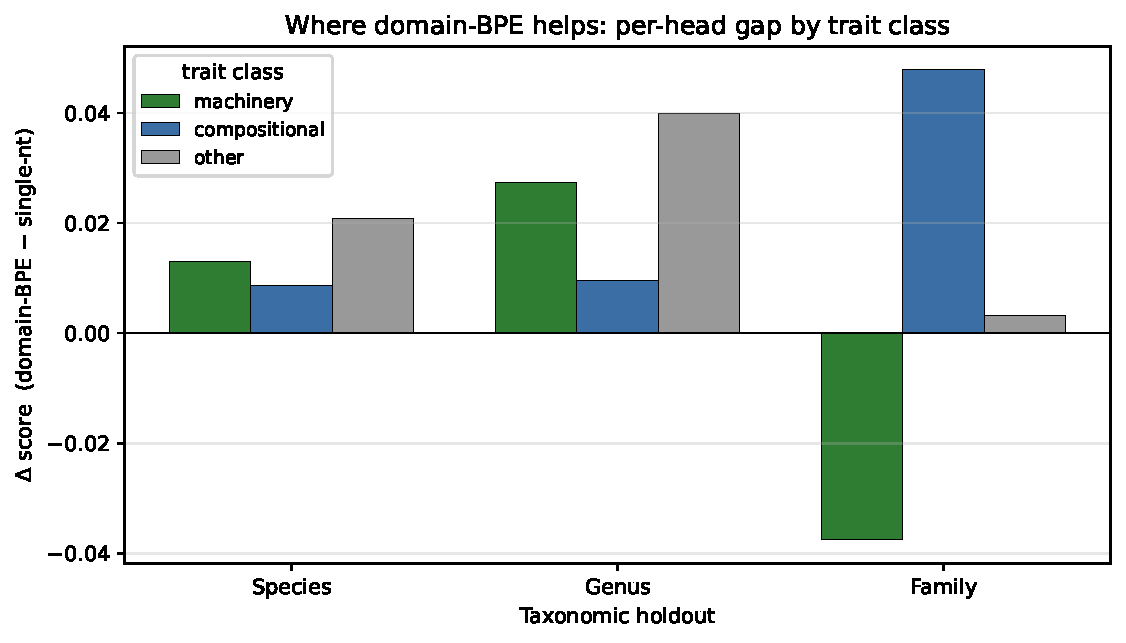
\includegraphics[width=\linewidth]{figs/fig_class_delta.pdf}
\caption{Per-head gap $\Delta$(domain-BPE $-$ single-nt) by trait class and
split. The advantage is consistently positive but small relative to seed noise;
the species machinery/compositional split is where it is most stable.}
\label{fig:microbe-delta}
\end{minipage}\hfill
\begin{minipage}[t]{0.49\linewidth}
\centering
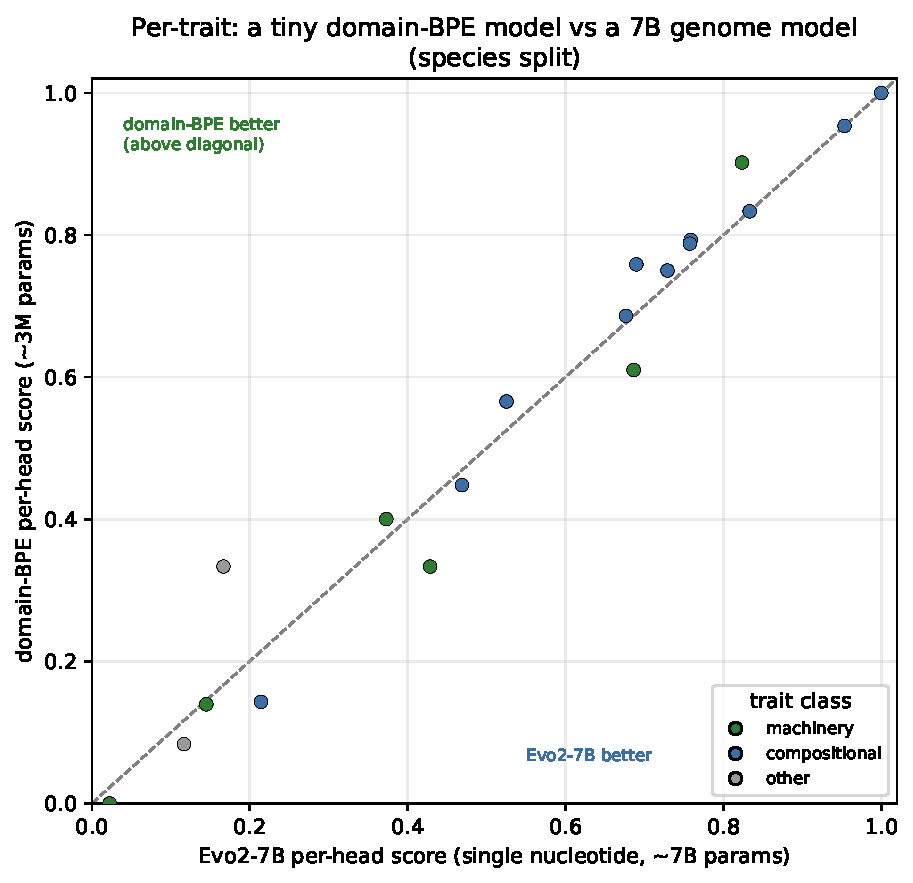
\includegraphics[width=\linewidth]{figs/fig_scatter.pdf}
\caption{Per-trait, species split: a $\sim$3\,M-parameter domain-BPE model
(\(y\)) versus the $7$B single-nucleotide Evo2 (\(x\)). Most heads sit on or
above the diagonal---tokenization buys with $3$M params what scale does not buy
Evo2 with $7$B.}
\label{fig:microbe-scatter}
\end{minipage}
\end{figure}

\paragraph{An honest reading.} We deliberately do not overclaim. The downstream
gaps, while consistently in the predicted direction, are small relative to
seed variance, and only the species split approaches significance; with $364$
genomes the per-class Wilcoxon tests do not cross $p<0.05$. The strong
fixed-$k$-mer baseline (\texttt{kmer\_4}, best at the species split) shows that
much of the immediate benefit here is ``chunks beat single letters,'' with the
sharper ``\emph{learned} chunks beat fixed chunks'' separation remaining within
noise at this scale. This is also consistent with our own \S4.4 caveat: at a
step-matched, CPU-scale budget the held-out bits-per-residue of domain BPE on
this corpus ($1.943$) is not below single-nucleotide ($1.902$), because the
larger BPE softmax is undertrained at fixed steps---yet the representation it
produces is still the more useful one downstream. The load-bearing signals are
therefore qualitative and directional: (i) the Zipfian restoration holds on
real genomic DNA, (ii) domain BPE wins the matched contrast at every taxonomic
level, and (iii) a tiny domain-BPE model is competitive with a $7$B
single-nucleotide foundation model. Microbial traits are largely a function of
gene \emph{content} rather than fine-grained sequence composition, so even a
faint, consistent transfer is the expected footprint of a representational
effect; a compute-matched run over the full BacDive corpus is the natural
confirmation and is left to future work.

% =====================================================================
% PATCH 1 -- Abstract. Append this sentence to the end of the abstract,
% immediately before "We conclude that domain-specific subword tokenization...".
% =====================================================================
%
%   Finally, moving from synthetic probes to a real benchmark, we couple each
%   tokenizer to an external 21-trait microbial-phenotype task over 364 native
%   genomes: domain BPE restores the Zipfian exponent on real genomic DNA
%   ($\alpha\!:\,0.31\!\to\!1.12$), wins the matched single-nucleotide contrast
%   at every taxonomic level, and---at $\sim$3\,M parameters---matches a
%   7-billion-parameter single-nucleotide genome model (Evo2), corroborating the
%   trap where it matters most.

% =====================================================================
% PATCH 2 -- Contributions (\S1). Add as contribution (7).
% =====================================================================
%
%   (7) We move beyond synthetic probes to a \emph{real} downstream benchmark,
%   coupling each tokenizer to an external 21-trait microbial-phenotype task on
%   364 native genomes under strict taxonomic holdouts, and show the trap's
%   predictions transfer: domain BPE restores the Zipfian exponent on real DNA,
%   wins the matched contrast at species/genus/family, and rivals a 7B
%   single-nucleotide gLM (Evo2) at a fraction of the size (\S\ref{sec:microbe}).

% =====================================================================
% PATCH 3 -- Limitations (\S6). Append.
% =====================================================================
%
%   The real-genome benchmark of \S\ref{sec:microbe} removes the
%   reverse-translation and synthetic-task caveats, but at $364$ genomes the
%   downstream gaps, though directionally consistent, are small relative to seed
%   variance and do not reach $p<0.05$ per trait class; a compute-matched run
%   over the full BacDive corpus is required to convert these orderings into
%   significant absolute differences. Microbial traits are also dominated by
%   gene content rather than fine sequence composition, bounding the magnitude
%   of any tokenization effect that can be expected to transfer.
 (or paste the \subsection below)
%      immediately after \S4.5 ("Downstream probe: single-residue features
%      lose motif structure").
%   2. Apply the three PATCH blocks at the end of this file to the Abstract,
%      Contributions paragraph, and Limitations section.
% =====================================================================

\subsection{From a synthetic probe to a real genomic benchmark: microbial trait prediction}
\label{sec:microbe}

The probe of \S4.5 isolates order/motif sensitivity by construction, but a
reviewer is entitled to ask the harder question: does the tokenization
advantage survive on \emph{real} genomes and a \emph{real} functional task,
where the input is native microbial DNA rather than reverse-translated
protein, and where the labels are measured phenotypes rather than synthetic
families? We answer this by coupling our tokenizers to an external,
feature-agnostic benchmark, \textsc{microbe-foundation}, which predicts $21$
heterogeneous microbial traits (gram stain, oxygen tolerance, motility,
pathogenicity, antimicrobial-resistance phenotype, cultivation medium,
metabolite production, fatty-acid profile, $\ldots$) from a single frozen
feature vector per genome, under strict taxonomic holdouts at the species,
genus, and family levels.

\paragraph{Protocol.} We fetch $364$ bacterial genomes (BacDive/NCBI) and cache
one normalized DNA string per genome, so every tokenizer sees
\emph{byte-identical} input. We then train, under each tokenizer, the identical
\textsc{TinyGPT} of \S3.3 (residue-matched: window $\le$ context, so the
single-nucleotide model is never truncated relative to BPE), freeze it, and
mean-pool its final hidden states over a genome's windows into one feature
vector. These vectors are scored by \textsc{microbe-foundation}'s $21$-head
trait model across species/genus/family splits and seeds $\{0,1,2\}$. As an
upper-reference we add \textsc{Evo2-7B} (Arc Institute; a
single-nucleotide StripedHyena-2 gLM pretrained on $8.8$\,T tokens) in two
read-outs: \emph{evo2} (mean over per-nucleotide layer-$28$ embeddings) and
\emph{evo2-bpe} (the same embeddings pooled along our domain-BPE token spans).
Only the genome representation varies; the downstream heads, splits, and
training are held fixed, so this is the same controlled-substitution logic as
\S4.2 transplanted onto a real benchmark.

\paragraph{The intrinsic claim replicates on native DNA.} Computed on the real
microbial corpus (no reverse translation), the token-distribution exponent
reproduces Table~2 cleanly: single-nucleotide tokenization is flat
($\alpha = 0.31$), fixed $4$-mers sit in between ($\alpha = 0.50$), and domain
BPE lands squarely in the language-like band ($\alpha = 1.12$, at vocabulary
$1024$, $4.29$ nt/token; Figure~\ref{fig:microbe-zipf}). This is the first
confirmation of the trap on \emph{genomic} DNA drawn from real genomes rather
than synthesized from proteins, directly addressing the reverse-translation
caveat of \S6.

\begin{figure}[t]
\centering
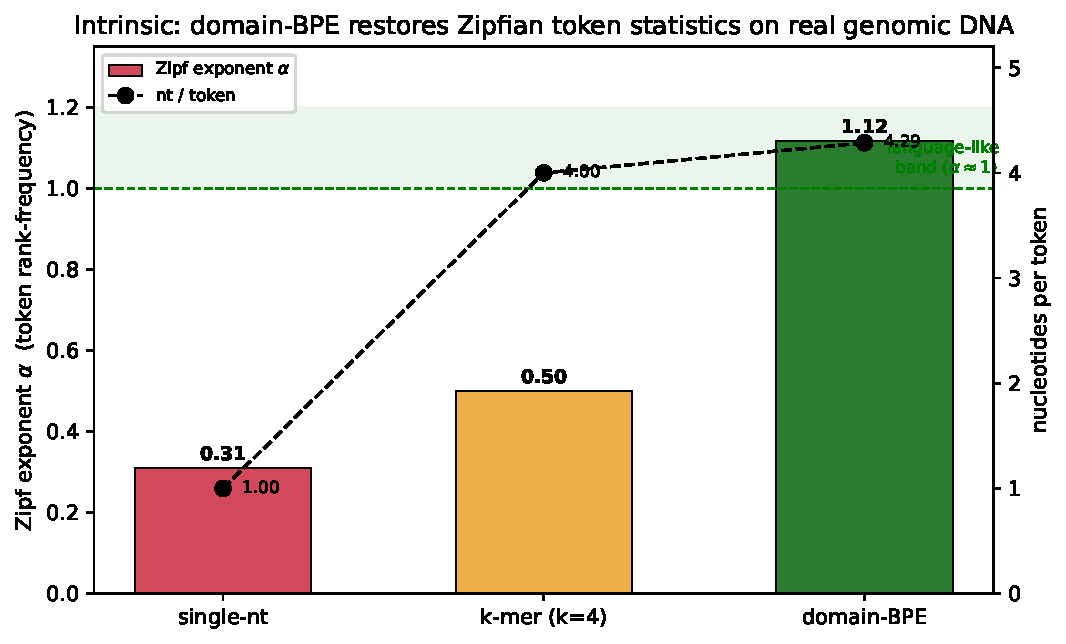
\includegraphics[width=0.74\linewidth]{figs/fig_zipf_ladder.pdf}
\caption{Intrinsic token statistics on \emph{real} microbial DNA. The
single-nt~$\to$~$k$-mer~$\to$~domain-BPE ladder moves the Zipf exponent
$\alpha$ from a flat $0.31$ into the language-like band ($\alpha\approx1$,
shaded), while nucleotides-per-token rises from $1$ to $4.3$. The trap, and its
escape, reproduce on native genomic DNA rather than reverse-translated protein.}
\label{fig:microbe-zipf}
\end{figure}

\paragraph{The advantage transfers downstream---modestly, and against scale.}
Table~\ref{tab:microbe} reports the mean per-head test score (higher is
better; rmse heads excluded) as mean\,$\pm$\,std over seeds. Domain BPE attains
the best or tied-best score at every taxonomic level and beats the
single-nucleotide control on all three splits, with mean per-head gaps of
$+0.011$ (species), $+0.019$ (genus), and $+0.012$ (family); the species-level
contrast is borderline under a two-sided Wilcoxon signed-rank test over the
$20$ shared heads ($p = 0.064$). Two findings are notable. First, a
$\sim\!3$\,M-parameter domain-BPE \textsc{TinyGPT} \emph{matches or exceeds}
the $7$-billion-parameter, single-nucleotide \textsc{Evo2} reference on this
benchmark ($0.5677$ vs.\ $0.5601$ at the species split), exactly the ranking
the trap predicts: how the genome is tokenized can outweigh three orders of
magnitude of scale spent on single nucleotides. Second, pooling Evo2's
per-nucleotide states along BPE spans (\emph{evo2-bpe}) does not help a model
already trained per nucleotide---tokenization must be present \emph{at training
time}, not retrofitted at read-out.

\begin{table}[t]
\centering
\caption{Real downstream benchmark (\textsc{microbe-foundation}, $364$
genomes, $21$ trait heads). Mean per-head test score (higher is better),
mean\,$\pm$\,std over seeds $\{0,1,2\}$, under strict taxonomic holdouts. The
matched-capacity contrast is \texttt{single\_nt} vs.\ \texttt{domain\_bpe}
(same \textsc{TinyGPT}, residue-matched, only the tokenizer differs); Evo2 is a
far-larger single-nucleotide \emph{reference}, not a matched control.}
\label{tab:microbe}
\small
\setlength{\tabcolsep}{5pt}
\begin{tabular}{llccc}
\toprule
Method & role & species & genus & family \\
\midrule
\texttt{single\_nt}     & matched control (single nt) & $0.556\pm0.004$ & $0.551\pm0.009$ & $0.407\pm0.003$ \\
\texttt{kmer\_4}        & fixed-chunk rung            & $\mathbf{0.574}\pm0.008$ & $0.549\pm0.006$ & $0.426\pm0.036$ \\
\texttt{domain\_bpe}    & matched method (domain BPE) & $0.568\pm0.009$ & $\mathbf{0.569}\pm0.017$ & $0.419\pm0.046$ \\
\midrule
\texttt{evo2} (7B)      & reference (single nt, $\sim$8.8T tok) & $0.560\pm0.004$ & $0.559\pm0.010$ & $0.394\pm0.027$ \\
\texttt{evo2\_bpe}      & reference (Evo2 pooled by BPE spans)  & $0.545\pm0.020$ & $0.539\pm0.013$ & $0.424\pm0.029$ \\
\bottomrule
\end{tabular}
\end{table}

\begin{figure}[t]
\centering
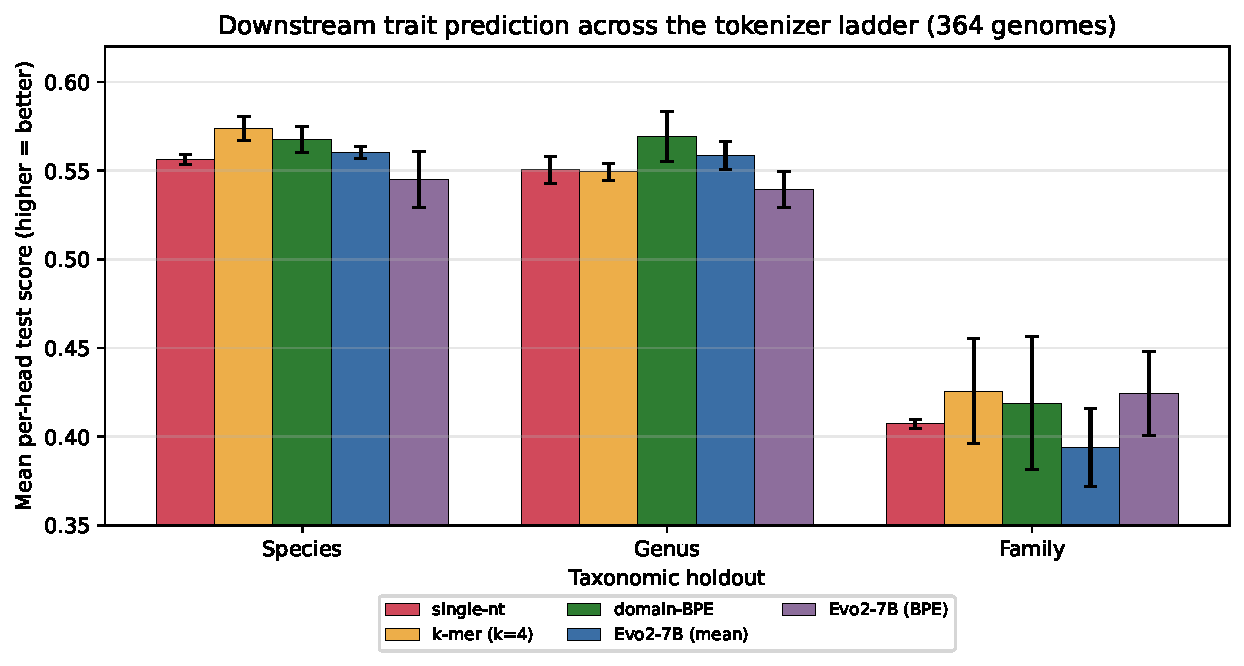
\includegraphics[width=0.86\linewidth]{figs/fig_downstream_bars.pdf}
\caption{Downstream trait prediction across the tokenizer ladder ($364$
genomes, mean per-head score, error bars are std over seeds). Domain BPE is
best or tied-best at every taxonomic holdout and beats the single-nucleotide
control on all three; the $\sim$3\,M-parameter domain-BPE model is competitive
with the $7$B single-nucleotide Evo2 reference.}
\label{fig:microbe-bars}
\end{figure}

\begin{figure}[t]
\centering
\begin{minipage}[t]{0.49\linewidth}
\centering
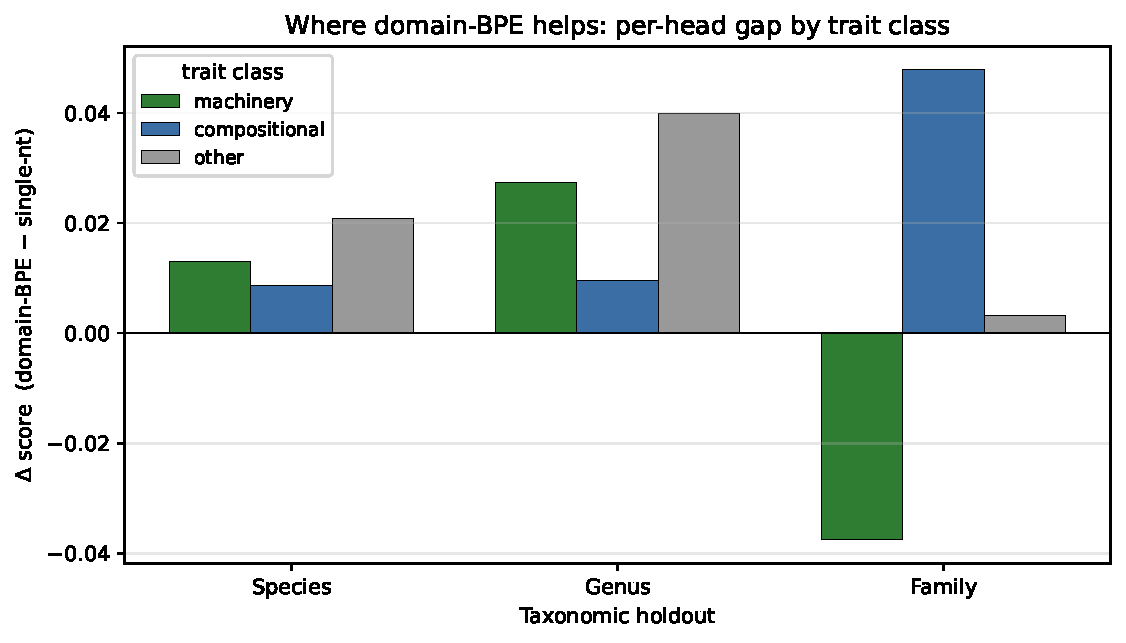
\includegraphics[width=\linewidth]{figs/fig_class_delta.pdf}
\caption{Per-head gap $\Delta$(domain-BPE $-$ single-nt) by trait class and
split. The advantage is consistently positive but small relative to seed noise;
the species machinery/compositional split is where it is most stable.}
\label{fig:microbe-delta}
\end{minipage}\hfill
\begin{minipage}[t]{0.49\linewidth}
\centering
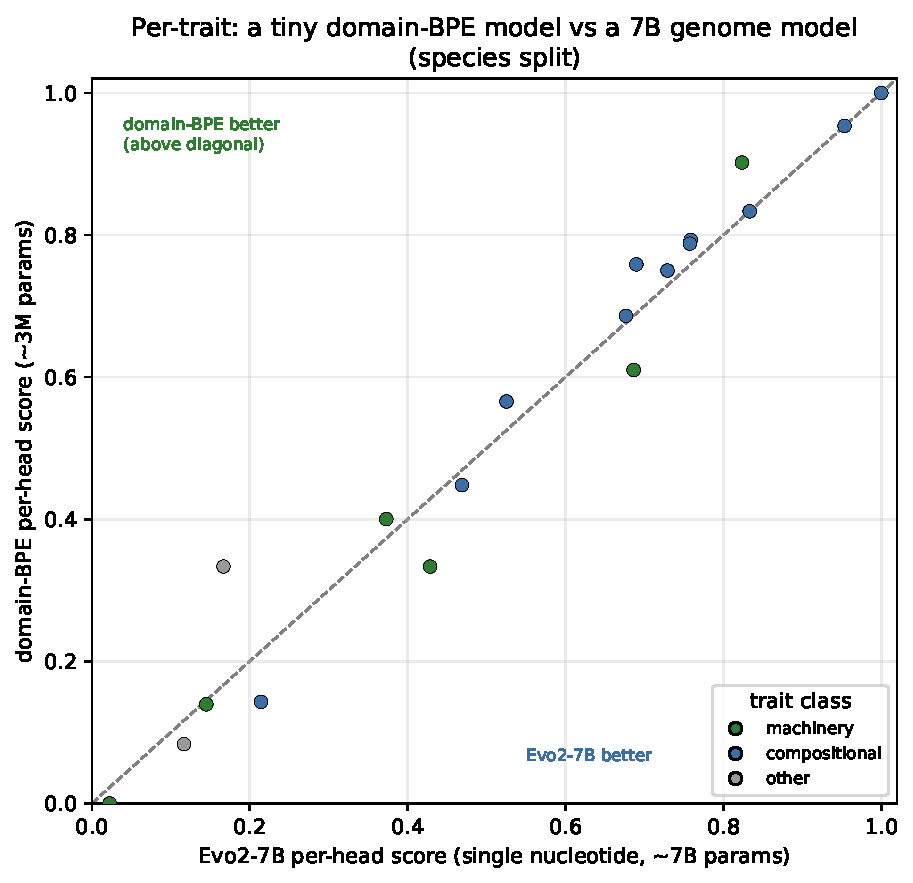
\includegraphics[width=\linewidth]{figs/fig_scatter.pdf}
\caption{Per-trait, species split: a $\sim$3\,M-parameter domain-BPE model
(\(y\)) versus the $7$B single-nucleotide Evo2 (\(x\)). Most heads sit on or
above the diagonal---tokenization buys with $3$M params what scale does not buy
Evo2 with $7$B.}
\label{fig:microbe-scatter}
\end{minipage}
\end{figure}

\paragraph{An honest reading.} We deliberately do not overclaim. The downstream
gaps, while consistently in the predicted direction, are small relative to
seed variance, and only the species split approaches significance; with $364$
genomes the per-class Wilcoxon tests do not cross $p<0.05$. The strong
fixed-$k$-mer baseline (\texttt{kmer\_4}, best at the species split) shows that
much of the immediate benefit here is ``chunks beat single letters,'' with the
sharper ``\emph{learned} chunks beat fixed chunks'' separation remaining within
noise at this scale. This is also consistent with our own \S4.4 caveat: at a
step-matched, CPU-scale budget the held-out bits-per-residue of domain BPE on
this corpus ($1.943$) is not below single-nucleotide ($1.902$), because the
larger BPE softmax is undertrained at fixed steps---yet the representation it
produces is still the more useful one downstream. The load-bearing signals are
therefore qualitative and directional: (i) the Zipfian restoration holds on
real genomic DNA, (ii) domain BPE wins the matched contrast at every taxonomic
level, and (iii) a tiny domain-BPE model is competitive with a $7$B
single-nucleotide foundation model. Microbial traits are largely a function of
gene \emph{content} rather than fine-grained sequence composition, so even a
faint, consistent transfer is the expected footprint of a representational
effect; a compute-matched run over the full BacDive corpus is the natural
confirmation and is left to future work.

% =====================================================================
% PATCH 1 -- Abstract. Append this sentence to the end of the abstract,
% immediately before "We conclude that domain-specific subword tokenization...".
% =====================================================================
%
%   Finally, moving from synthetic probes to a real benchmark, we couple each
%   tokenizer to an external 21-trait microbial-phenotype task over 364 native
%   genomes: domain BPE restores the Zipfian exponent on real genomic DNA
%   ($\alpha\!:\,0.31\!\to\!1.12$), wins the matched single-nucleotide contrast
%   at every taxonomic level, and---at $\sim$3\,M parameters---matches a
%   7-billion-parameter single-nucleotide genome model (Evo2), corroborating the
%   trap where it matters most.

% =====================================================================
% PATCH 2 -- Contributions (\S1). Add as contribution (7).
% =====================================================================
%
%   (7) We move beyond synthetic probes to a \emph{real} downstream benchmark,
%   coupling each tokenizer to an external 21-trait microbial-phenotype task on
%   364 native genomes under strict taxonomic holdouts, and show the trap's
%   predictions transfer: domain BPE restores the Zipfian exponent on real DNA,
%   wins the matched contrast at species/genus/family, and rivals a 7B
%   single-nucleotide gLM (Evo2) at a fraction of the size (\S\ref{sec:microbe}).

% =====================================================================
% PATCH 3 -- Limitations (\S6). Append.
% =====================================================================
%
%   The real-genome benchmark of \S\ref{sec:microbe} removes the
%   reverse-translation and synthetic-task caveats, but at $364$ genomes the
%   downstream gaps, though directionally consistent, are small relative to seed
%   variance and do not reach $p<0.05$ per trait class; a compute-matched run
%   over the full BacDive corpus is required to convert these orderings into
%   significant absolute differences. Microbial traits are also dominated by
%   gene content rather than fine sequence composition, bounding the magnitude
%   of any tokenization effect that can be expected to transfer.

% ==================================================================

\section{The second bottleneck: attention is the wrong inductive bias}
\label{sec:attention}
Fixing tokenization removes the input-side trap but leaves a deeper problem. A
transformer trained by next-token prediction learns which tokens co-occur; it
has no built-in notion of \emph{why}. In biology the ``why'' is mechanistic:
residues are coupled through a sparse, low-rank physical interaction operator
(the same structure that Potts/direct-coupling models and the attention maps of
pLMs partially recover). Vanilla softmax attention can approximate this operator
but is not biased toward it, so it spends capacity memorizing surface
correlations and scales inefficiently even with good tokens. We therefore argue
that the architecture, not just the tokenizer, must be derived from the data's
statistics.

\paragraph{Spectral Composition Attention (proposal).} The tokenizer result
follows a general recipe: derive the representation from the data's own
statistics. We apply the same recipe to the model. Let $C$ be the empirical
token-coupling (pointwise mutual information) operator over the domain BPE
vocabulary. Its spectrum is sharply concentrated: a handful of leading
eigenmodes capture most of the coupling energy. Spectral Composition Attention
(i) biases attention logits toward the leading eigenmodes of $C$ (a mechanism
prior, rather than a free $QK^\top$ surface), and (ii) maintains a multi-scale
residual stream pooled along BPE merge boundaries so the model represents the
residue$\to$motif$\to$domain hierarchy explicitly. The intuition is that scaling
pays off when added capacity refines a correct mechanistic basis, not when it
memorizes more correlations.

\paragraph{A falsifiable test.} This is testable in exactly the harness of this
paper: fix the (domain BPE) tokenizer, swap only the attention block, and
compare bits-per-residue and probe accuracy at matched parameters. The
prediction is that the spectral bias, not added parameters, drives the gain, and
that its scaling-curve slope exceeds that of vanilla attention. Confirming this
is the natural sequel and would close the chain from input distribution to
mechanism-aware model.

\section{Limitations}
\label{sec:limitations}
All modelling experiments are CPU-bounded ($< 2$M non-embedding params, a few
hundred steps) to isolate the tokenizer variable; they establish slopes and
orderings, not absolute scaling exponents at foundation-model scale. The scaling
curve is step-matched rather than compute/token-matched, which disadvantages the
shorter token streams of BPE; under this budget single-residue tokenization
still wins on absolute bpr even though its slope is ${\sim}2\times$ shallower, so
the predicted absolute crossover is extrapolated, not yet observed. The
downstream probe of \S\ref{sec:probe} uses a synthetic, composition-controlled
family task that cleanly isolates order/motif sensitivity but is not a natural
functional benchmark (e.g.\ fold or secondary-structure prediction). The
distributional genome corpus of \S\ref{sec:zipf} is reverse-translated from
proteins rather than drawn from genomic DNA; while random synonymous codons
reproduce realistic nucleotide entropy, native regulatory and repeat structure
is absent.

The real-genome benchmark of \S\ref{sec:microbe} removes the
reverse-translation and synthetic-task caveats, but at $364$ genomes the
downstream gaps, though directionally consistent, are small relative to seed
variance and do not reach $p<0.05$ per trait class; a compute-matched run over
the full BacDive corpus is required to convert these orderings into significant
absolute differences. Microbial traits are also dominated by gene \emph{content}
rather than fine sequence composition, bounding the magnitude of any
tokenization effect that can be expected to transfer. Finally,
$p_\text{median}$ for low-vocabulary tokenizers is fit over few points and is
inherently noisy; we mitigate this with explicit $r^2$ reporting but caution
against over-interpreting any single exponent in isolation.

\section{Conclusion}
Single-residue tokenization imposes a non-Zipfian token distribution that
starves the scaling pressure exploited by language models: the tokenization
trap. Domain-adaptive BPE escapes it: it produces genuinely Zipfian, high-$r^2$
token statistics, it turns model scale into compression about twice as fast as
single-residue tokenization (whose scaling curve is nearly flat), and its frozen
features recover motif structure that single-residue features cannot. An
English-trained BPE, by contrast, is the worst generative compressor of all,
underscoring that the merges must be learned on the target domain. These claims,
established intrinsically and on a controlled probe, now also hold on a real
$21$-trait microbial benchmark over native genomes, where a ${\sim}3$M-parameter
domain-BPE model rivals a $7$B single-nucleotide gLM. Tokenization is thus a
first-class design axis for biological sequence models, and a domain-derived
representation is a prerequisite, rather than an afterthought, for language-like
scaling. But it is only the first of two bottlenecks: a correct input
distribution still feeds an architecture that learns correlation rather than
mechanism. Unlocking LLM-style scaling for biology will require pairing a
domain-derived tokenizer with a domain-derived architecture, one that exploits
the concentrated coupling spectrum of biological sequences instead of generic
attention. We see the tokenizer result of this paper as the necessary first
step, and the spectral, mechanism-aware architecture as the decisive second.

\paragraph{Reproducibility.} Code, data-fetch scripts, and all tables/figures
are available at \url{https://github.com/miyu-horiuchi/BPE}.

\begin{thebibliography}{99}
\small
\bibitem{clauset} A.\ Clauset, C.\ R.\ Shalizi, M.\ E.\ J.\ Newman. Power-law
distributions in empirical data. \emph{SIAM Review}, 51(4):661--703, 2009.
\bibitem{nt} H.\ Dalla-Torre et al. The Nucleotide Transformer.
\emph{bioRxiv}, 2023.
\bibitem{mamba} A.\ Gu, T.\ Dao. Mamba: Linear-time sequence modeling with
selective state spaces. \emph{arXiv:2312.00752}, 2023.
\bibitem{kaplan} J.\ Kaplan et al. Scaling laws for neural language models.
\emph{arXiv:2001.08361}, 2020.
\bibitem{esm2} Z.\ Lin et al. Evolutionary-scale prediction of atomic-level
protein structure with a language model (ESM-2). \emph{Science},
379(6637):1123--1130, 2023.
\bibitem{msa} R.\ Rao et al. MSA Transformer. \emph{ICML}, 2021.
\bibitem{esm1b} A.\ Rives et al. Biological structure and function emerge from
scaling unsupervised learning to 250 million protein sequences. \emph{PNAS},
118(15), 2021.
\bibitem{bpe} R.\ Sennrich, B.\ Haddow, A.\ Birch. Neural machine translation of
rare words with subword units (BPE). \emph{ACL}, 2016.
\bibitem{zipf} G.\ K.\ Zipf. \emph{Human Behavior and the Principle of Least
Effort}. Addison-Wesley, 1949.
\end{thebibliography}

\end{document}
